\chapter{Results}\label{sec:results}
This chapter collects the results along the stages of this thesis project. In section \ref{subsec:fourvsfive} is a comparison between the personality model of choice and the base project's, so the interested user can translate the personality-based results to either works. In section \ref{subsec:dataresults} are collected the results from the data collection. The output from the Genetic Algorithm will be discussed in section \ref{sec:gares}. Lastly, the results from the evaluation process will be discussed in section \ref{sec:reeval}.
\section{Comparison of Personality Models}\label{subsec:fourvsfive}
It has been mentioned in section \ref{subsubsec:big5} that the original project this thesis is basing itself on adopted the Big Five as personality model. Due to its complexity, it is harder to be applied in this context, therefore a comparison of the two models, the Big Five and the Four Temperaments, had to be searched upon. Unfortunately, such direct comparison does not seem to be directly available. We then compare Galen-Hippocrates' four types to Keirsey's and then to Myers-Briggs.\\
It is easy to find association between Keirsey's types, Galen-Hippocrates' and Myer-Briggs', as for example in Keirsey's book\cite{keirsey1998please}.  In table \ref{tab:keirsey} we can see a summary of those types, and how they are equated to each other.
\begin{table}[H]
	\caption{Comparison of Galen-Hippocrates' Four Temperaments with Keirsey's Four Temperaments and Myer-Briggs personality types, as from \cite{keirsey1998please}.}
    \centering
    \scriptsize
    \begin{tabular}{|c|c|c|c|c|}
    \hline
    Models & \multicolumn{4}{|c|}{Types} \\
		\hline
        \hline
        Galen-Hippocrates & Sanguine & Choleric & Melancholic & Phlegmatic\\
        \hline
        Keirsey & Artisan & Idealist & Guardian & Rational\\
        \hline
        Myer-Briggs & E\textbf{S}T\textbf{P} & E\textbf{NF}J & E\textbf{NT}J & E\textbf{S}T\textbf{J} \\
       				& I\textbf{S}T\textbf{P} & I\textbf{NF}J & I\textbf{NT}J & I\textbf{S}T\textbf{J} \\
                    & E\textbf{S}F\textbf{P} & E\textbf{NF}P & E\textbf{NT}P & E\textbf{S}F\textbf{J} \\
                    & I\textbf{S}F\textbf{P} & I\textbf{NF}P & I\textbf{NT}P & I\textbf{S}F\textbf{J} \\
        \hline
        Common traits Myers-Bryggs & SP & NF & NT & SJ \\
        \hline
    \end{tabular}
    \label{tab:keirsey}
\end{table}
There has been a study to correlate the Myers-Briggs types to the Big 5, and the results are described in \cite{mccrae1989reinterpreting}, and shown in table \ref{tab:big5mb}. The results were collected by a population of 267 men and 201 women, and it was found that the correlation values for men and women have negligible difference. Hence, we can just as well consider the results gathered from the men population, and consider it valid.
Given table \ref{tab:keirsey}, we can easily define a table with the probability of being any of the Myer-Briggs types, given the Galen-Hippocrates', and it can be seen in table \ref{tab:prob-myers-galen}.
\begin{table}[H]
    \caption{Correlation of Big 5 factors with Myer-Briggs (data from \cite{mccrae1989reinterpreting}).}
    \centering
    \scriptsize
    \begin{tabular}{|c|c|c|c|c|}
    \hline
    \multirow{2}{4em}{Big 5} & \multicolumn{4}{|c|}{Myer-Briggs} \\
    \cline{2-5}
         & E-I & S-N & T-F & J-P\\
        \hline
        \hline
        Neuroticism & 0.16 & -0.06 & 0.06 & 0.11\\
        \hline
        Extraversion & -0.74 & 0.10 & 0.19 & 0.15 \\
        \hline
       	Openness & 0.03 & 0.72 & 0.02 & 0.30 \\
        \hline
		Agreeableness & -0.03 & 0.04 & 0.44 & -0.06 \\
        \hline
		Conscientiousness & 0.08 & -0.15 & -0.15 & -0.49 \\
        \hline
    \end{tabular}
    \label{tab:big5mb}
\end{table}
\begin{table}[H]
	\caption{Probability of each Myer-Briggs preferences given the Galen-Hippocrates' type.}
   	\centering
    \scriptsize
    \begin{tabular}{|c||c|c||c|c||c|c||c|c|}
    	\hline
    	& E & I & N & S & F & T & J & P\\
      	\hline
        Choleric & 0,5 & 0,5 & 1 & 0 & 1 & 0 & 0,5 & 0,5\\
		\hline
        Sanguine & 0,5 & 0,5 & 0 & 1 & 0,5 & 0,5 & 0 & 1\\
        \hline
		Phlegmatic & 0,5 & 0,5 & 0 & 1 & 0,5 & 0,5 & 1 & 0\\
		\hline
        Melancholic & 0,5 & 0,5 & 1 & 0 & 0 & 1 & 0,5 & 0,5\\
        \hline
    \end{tabular}
    \label{tab:prob-myers-galen}
\end{table}
\begin{table}[H]
    \caption{Extension of table \ref{tab:big5mb}, with clarification of the preferences scale.}
	\centering
    \scriptsize
    \begin{tabular}{|c||c|c||c|c||c|c||c|c|}
    	\hline
    	& E & I & N & S & F & T & J & P\\
        \hline
		Openness & 0 & 0,03 & 0,72 & 0 & 0,02 & 0 & 0 & 0,3\\
        \hline
		Conscientiousness & 0 & 0,08 & 0 & 0,15 & 0 & 0,15 & 0,49 & 0\\
        \hline
		Extraversion & 0,74 & 0 & 0,1 & 0 & 0,19 & 0 & 0 & 0,15\\
		\hline
		Agreeableness & 0,03 & 0 & 0,04 & 0 & 0,44 & 0 & 0,06 & 0\\
        \hline
		Neuroticism & 0 & 0,16 & 0 & 0,06 & 0,06 & 0 & 0 & 0,11\\
		\hline
    \end{tabular}
    \label{tab:correlationExtended}
\end{table}
Table \ref{tab:correlationExtended} shows the same values as in table \ref{tab:big5mb}, just written in a way that emphasises the correlation values of each of the Myer-Briggs preferences, given the Big 5 types.\\
Finally, the relation between tables \ref{tab:prob-myers-galen} and \ref{tab:correlationExtended} can be calculated.
Let $J$ be a matrix containing the values in table \ref{tab:prob-myers-galen}, and $K$ be a matrix containing the values in table \ref{tab:correlationExtended}. Then it can be said that $$R=JK^T$$ where $R$ shows the correlation between the Four Temperaments and the Big 5, and which values can be seen in table \ref{tab:results}.
\begin{table}[H]
    \caption{Correlation between the Four Temperaments and Big 5.}
    \scriptsize
	\centering
	\begin{tabular}{|c|c|c|c|c|c|}
    	\hline
		& Openness& Conscientiousness & Extraversion & Agreeableness & Neuroticism\\
        \hline
		Choleric & 0,905 & 0,285 & 0,735 & 0,525 & 0,195\\
        \hline
		Sanguine & 0,325 & 0,265 & 0,615 & 0,235 & 0,28\\
        \hline
		Phlegmatic & 0,025 & 0,755 & 0,465 & 0,295 & 0,17\\
        \hline
		Melancholic & 0,885 & 0,435 & 0,545 & 0,085 & 0,135\\
		\hline		
	\end{tabular}
    \label{tab:results}
\end{table}
\begin{figure}[H]
\centering
	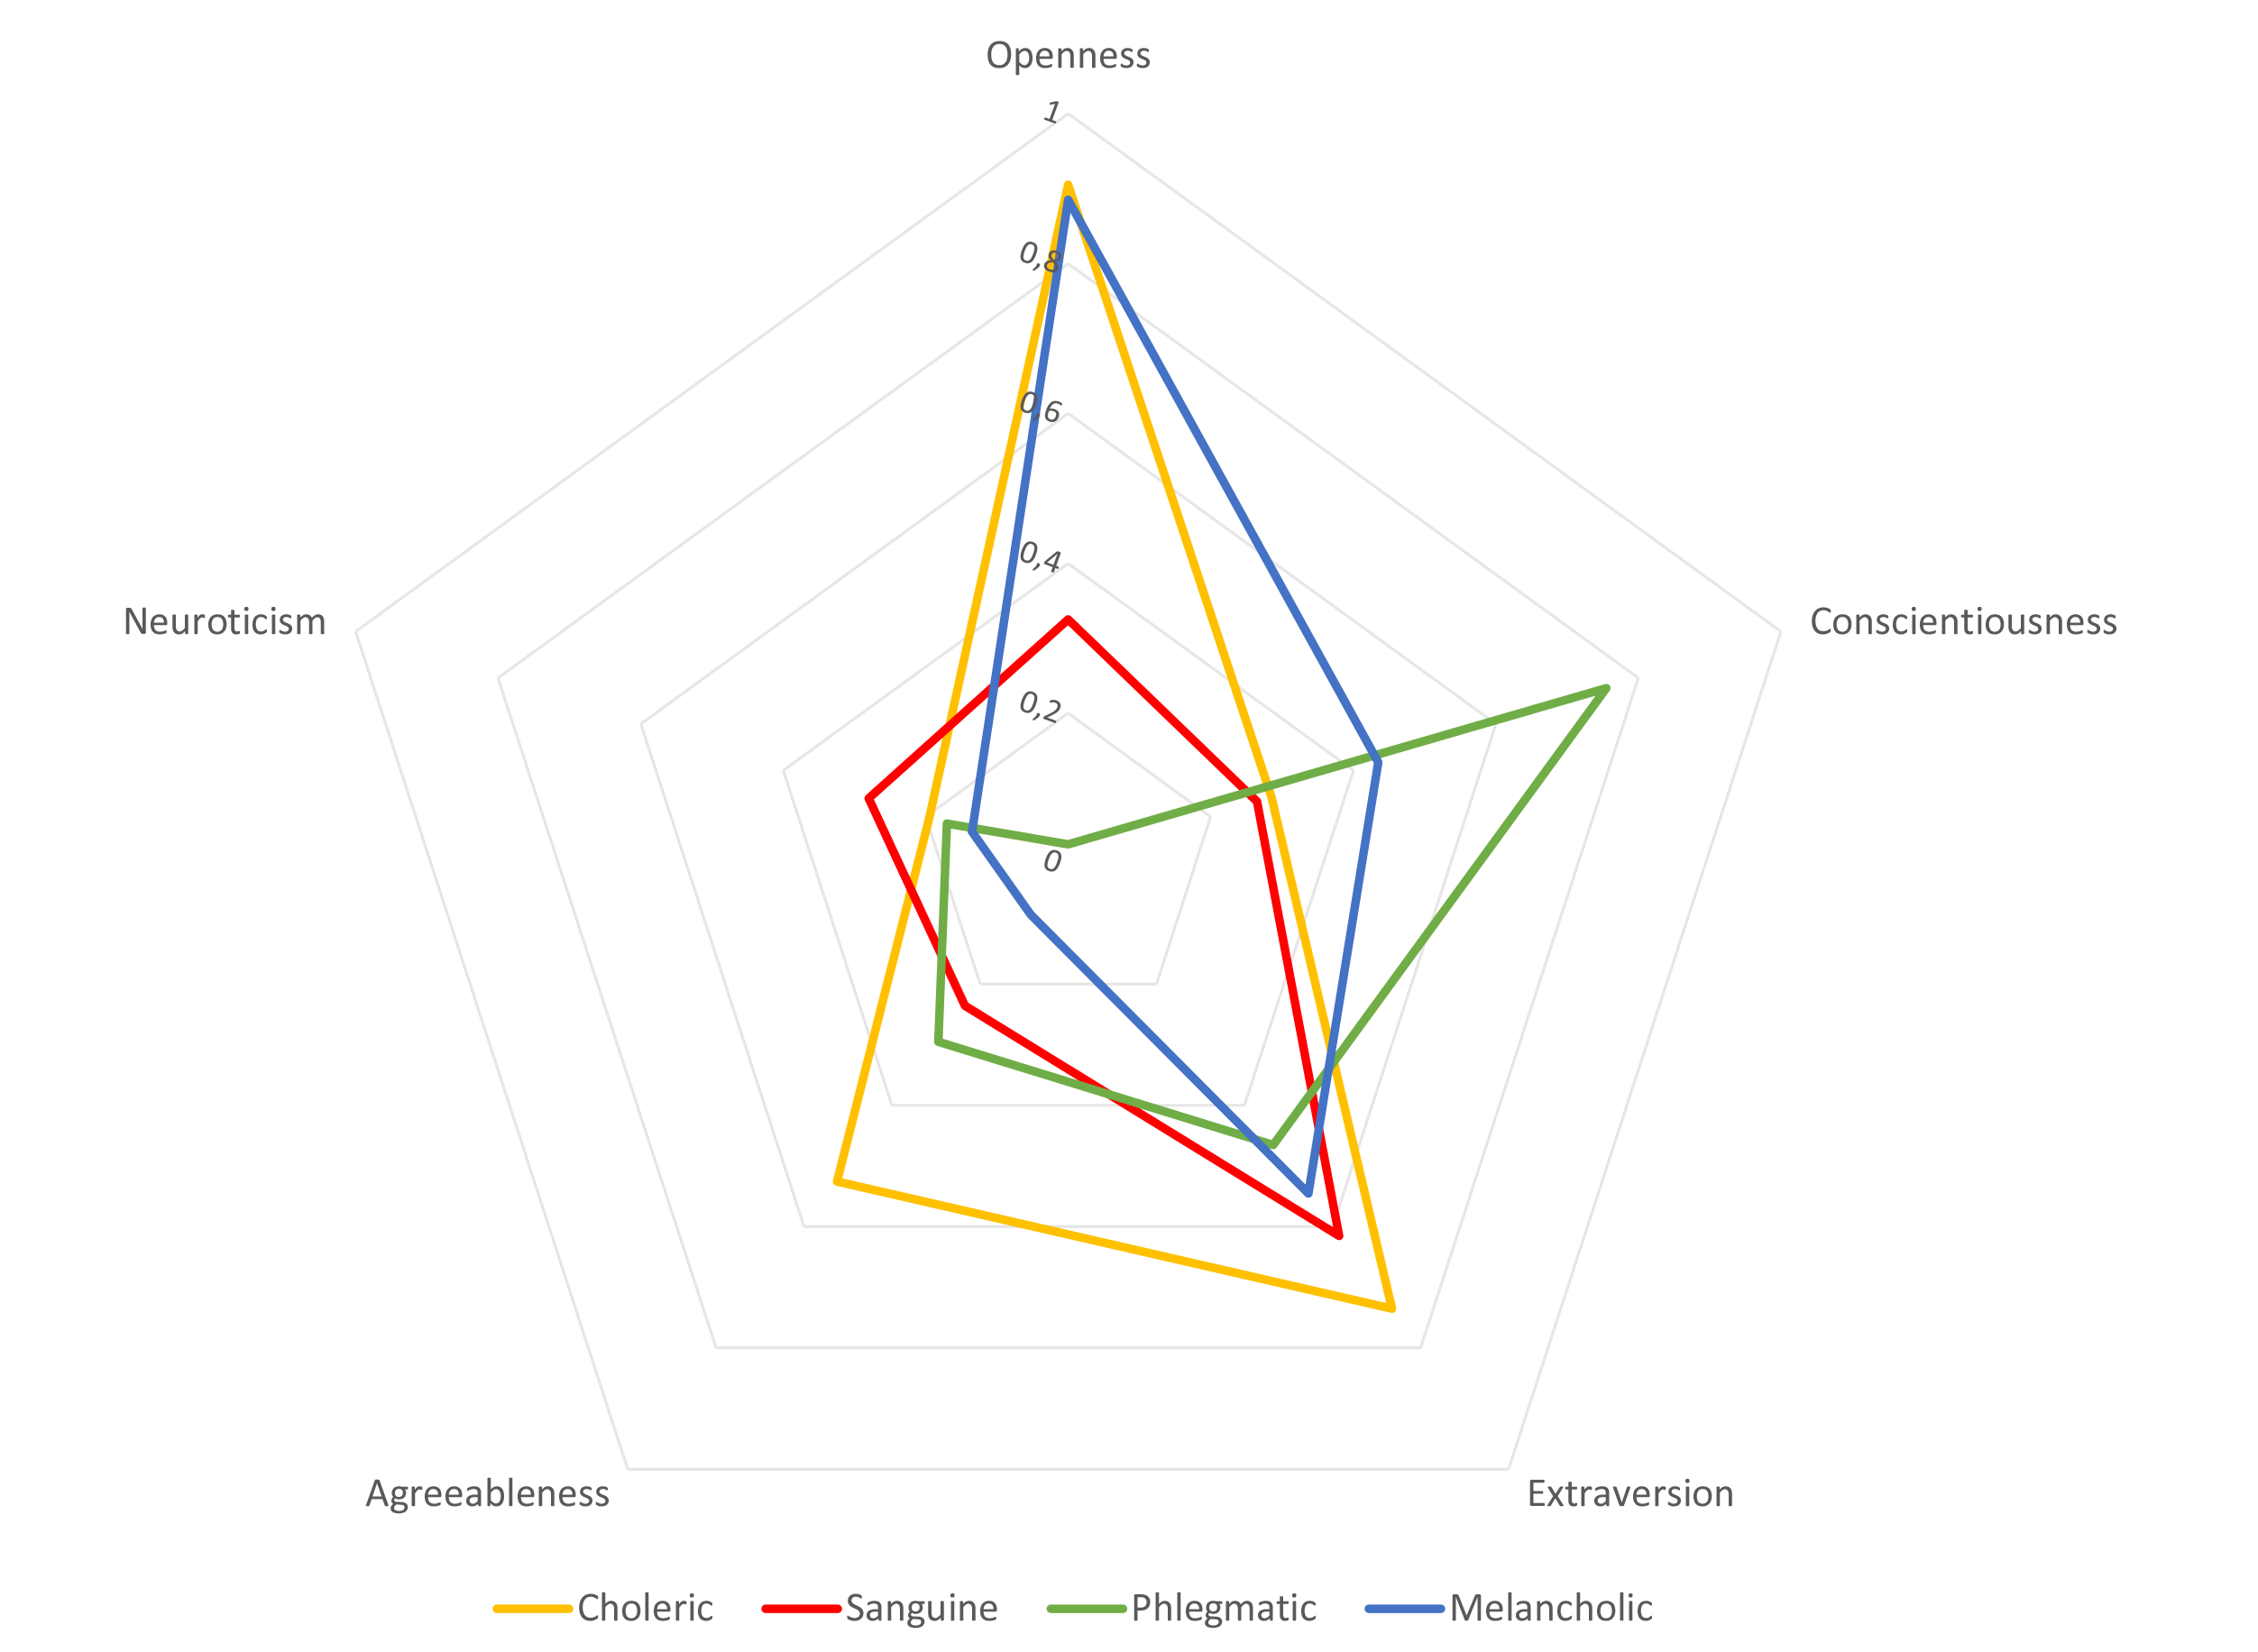
\includegraphics[scale=0.15]{figure/graph1}
    \caption{Correlation between the Four Temperaments and Big 5 factors.}
    \label{fig:all4}
\end{figure}
In figure \ref{fig:all4} we can see the comparison between all the temperaments, while in figure \ref{fig:4t-big5} we can see the temperaments singularly.
Since the old project allows only three settings for each of the Big 5 traits (low, medium, high), we thought it could be useful to normalize the results in \ref{tab:results} in a scale 0-2, and consequently round up at the closest integer. The results are shown in table \ref{tab:normalized}.
\begin{table}[H]
	\caption{Correlation of Big 5 factors with Myer-Briggs (table \ref{tab:results}) normalized to 2.}
	\centering
    \scriptsize
    \begin{tabular}{|c|c|c|c|c|c|}
    	\hline
    	& Openness & Conscientiousness & Extraversion & Agreeableness & Neuroticism\\
        \hline
        Choleric & 2 & 1 & 1 & 1 & 0\\
        \hline
		Sanguine & 1 & 1 & 1 & 0 & 1\\
		\hline
		Phlegmatic & 0 & 2 & 1 & 1 & 0\\
		\hline
		Melancholic & 2 & 1 & 1 & 0 & 0\\
		\hline
    \end{tabular}
    \label{tab:normalized}
\end{table}
The conclusion that can be drawn from looking at the results, is that the Neuroticism value is mostly irrelevant for the Four Temperaments model, nonetheless, we believe it might influence the game play, proving in this way that the chosen personality model is not complete to represent human behaviour properly in the general game play field. However, the magnitude of data collected for this project reduced the option of utilising any other complicated model, which would maybe be more suitable for modeling human behaviour in games.
\begin{figure}[ht!]
\centering
    \subfloat[Choleric graph][Choleric] {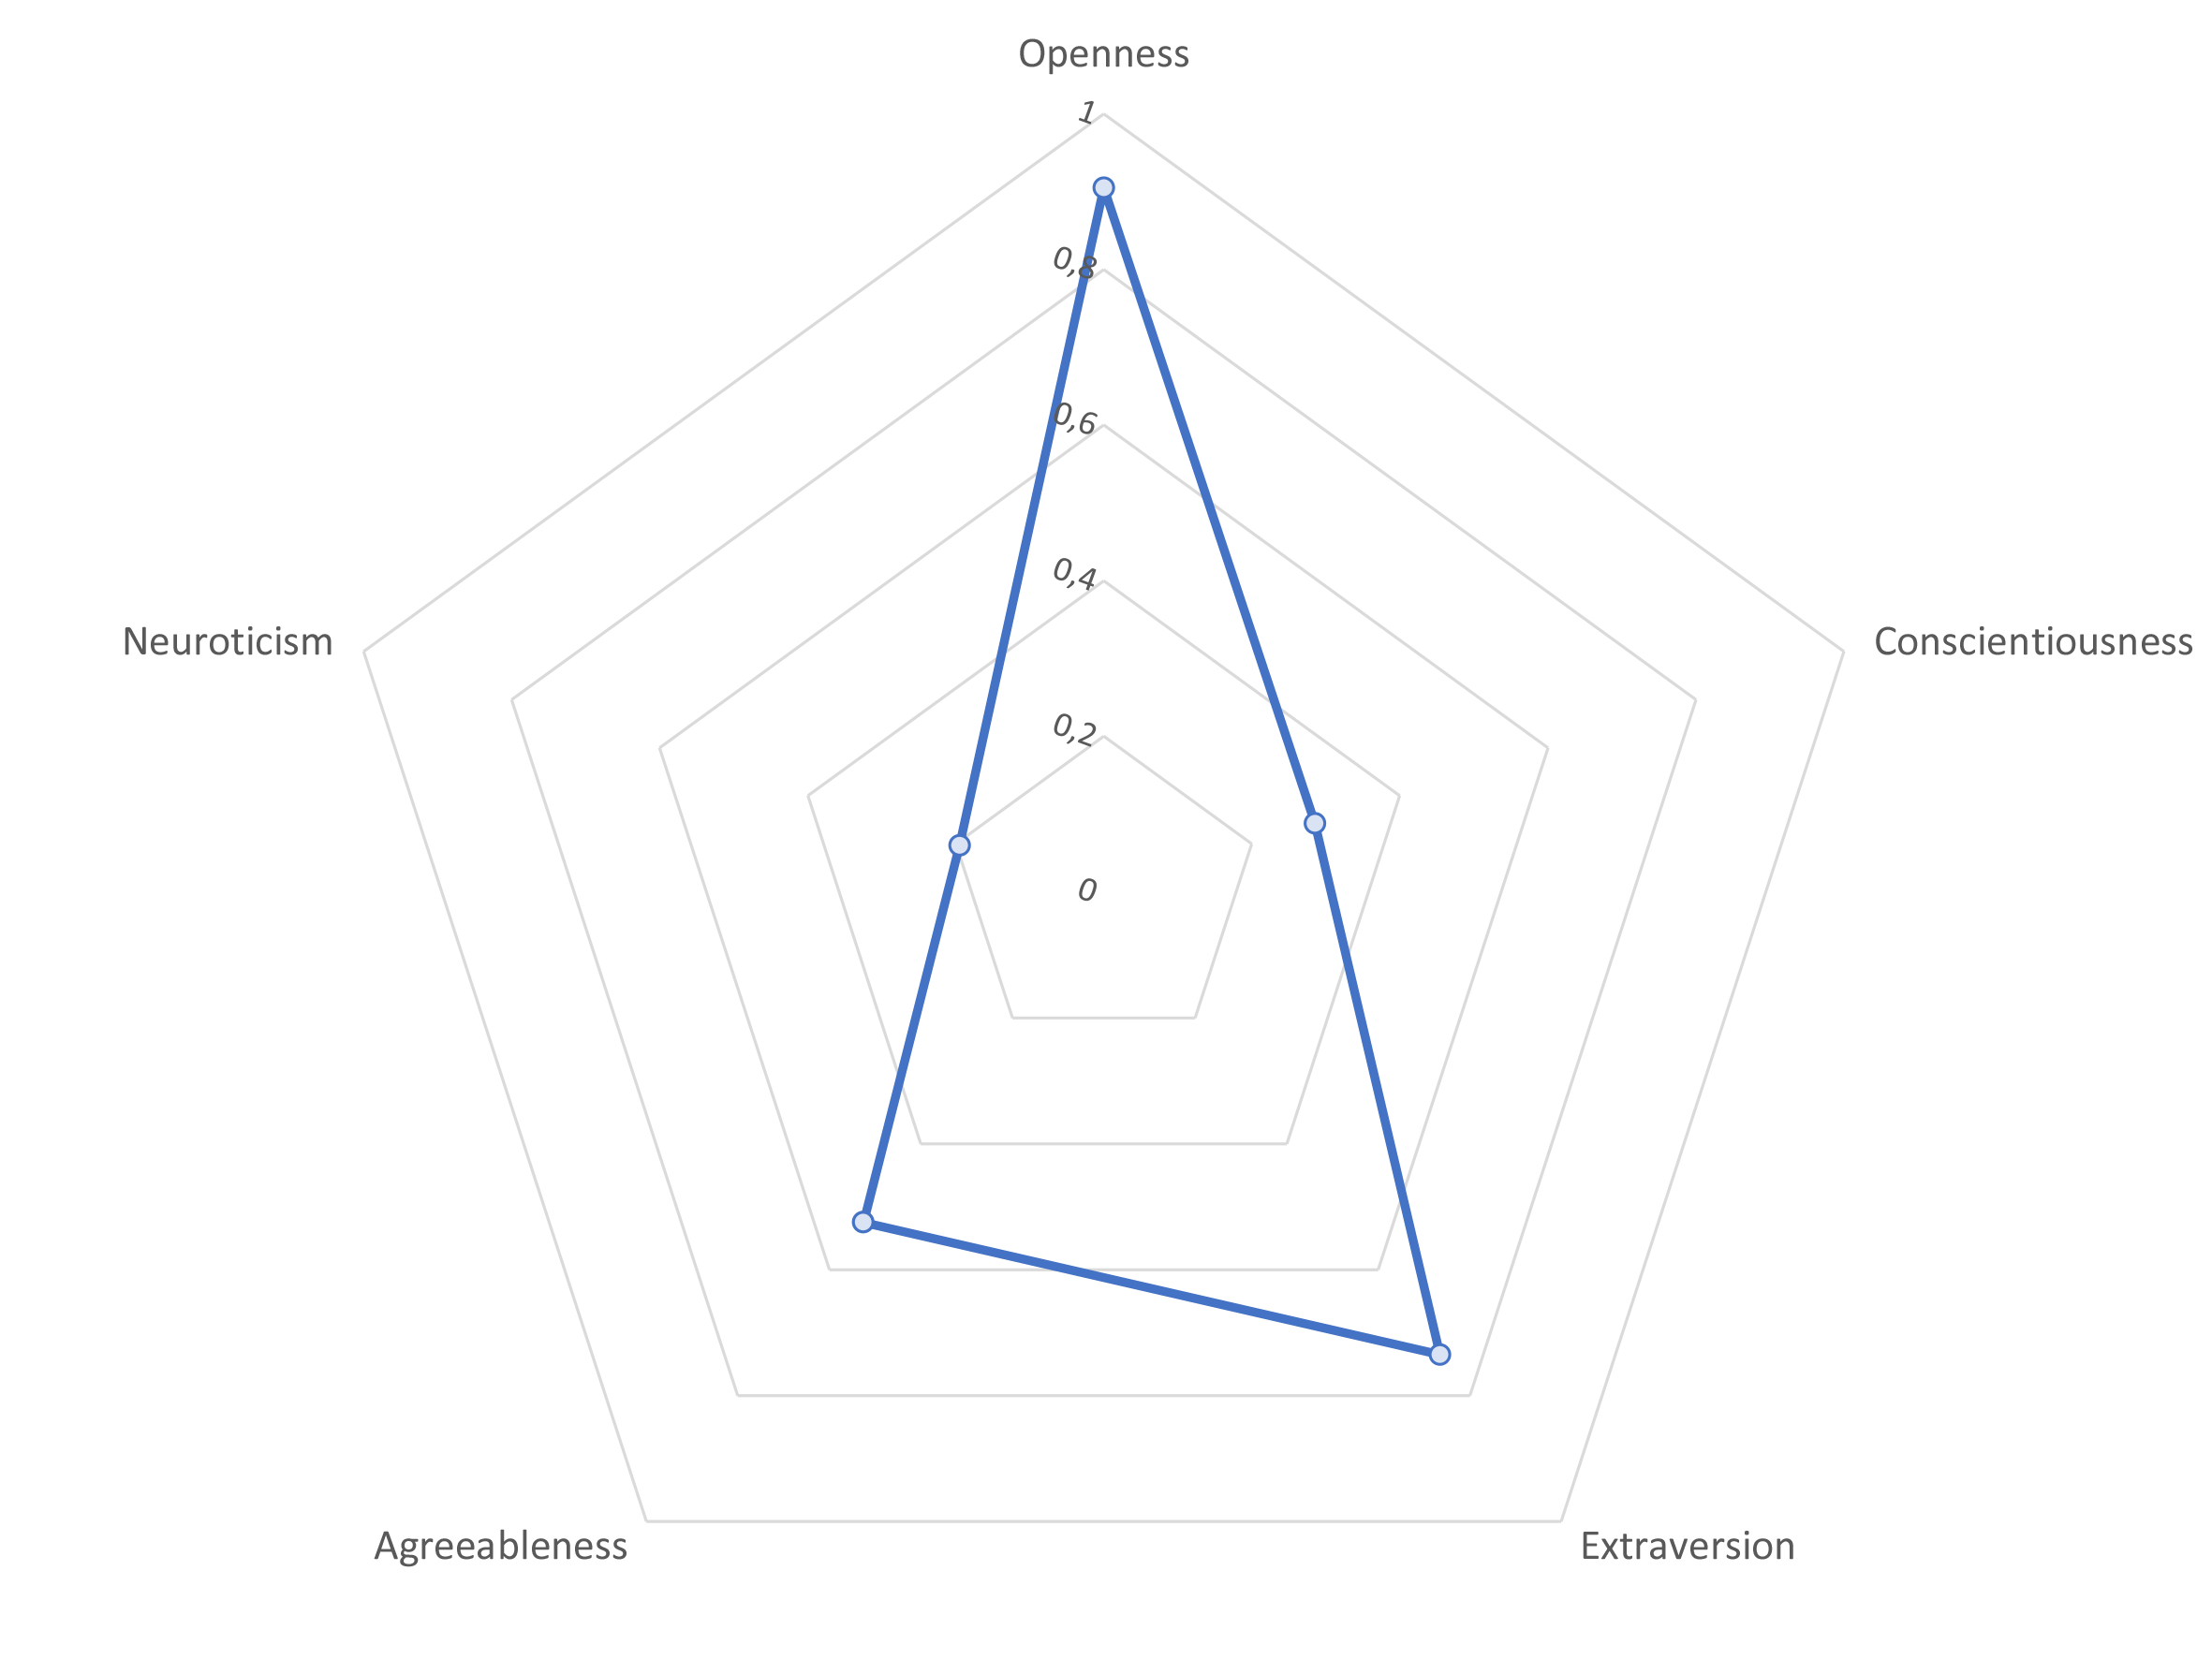
\includegraphics[scale=0.35]{figure/graph2_choleric}}
    \subfloat[Melancholic graph][Melancholic]{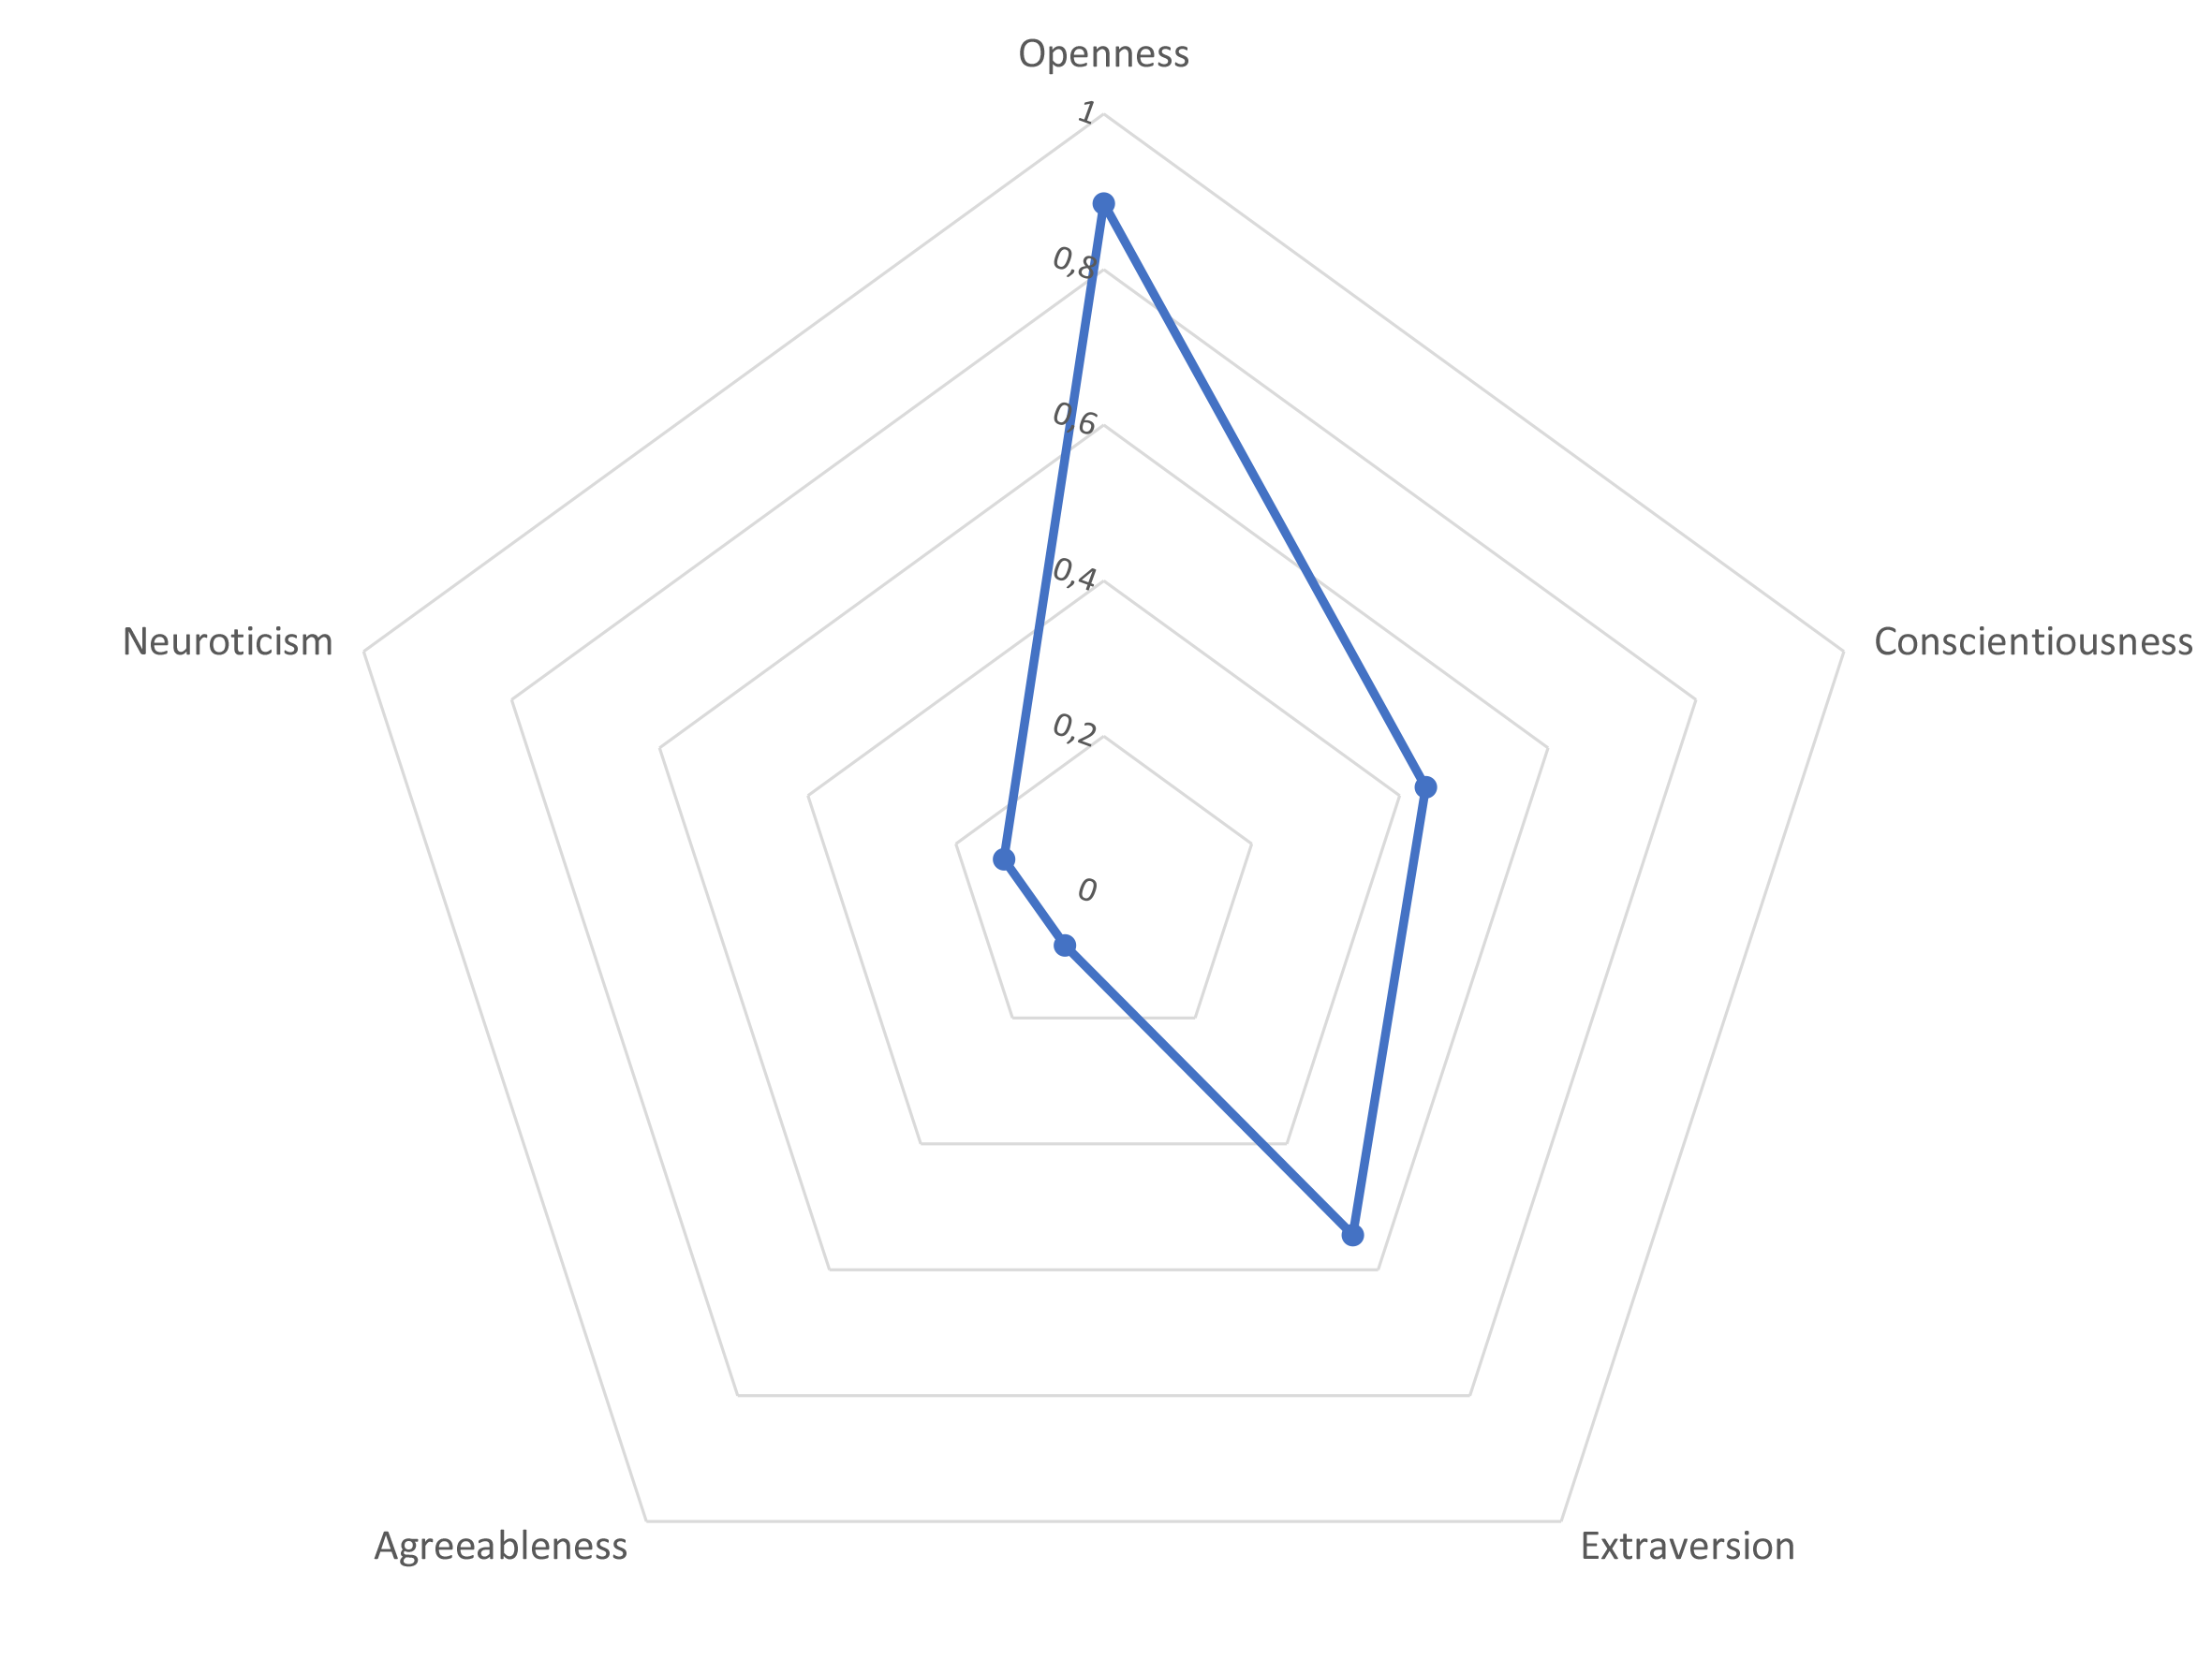
\includegraphics[scale=0.35]{figure/graph5_melancholic}}
    \qquad
    \subfloat[Sanguine graph][Sanguine]{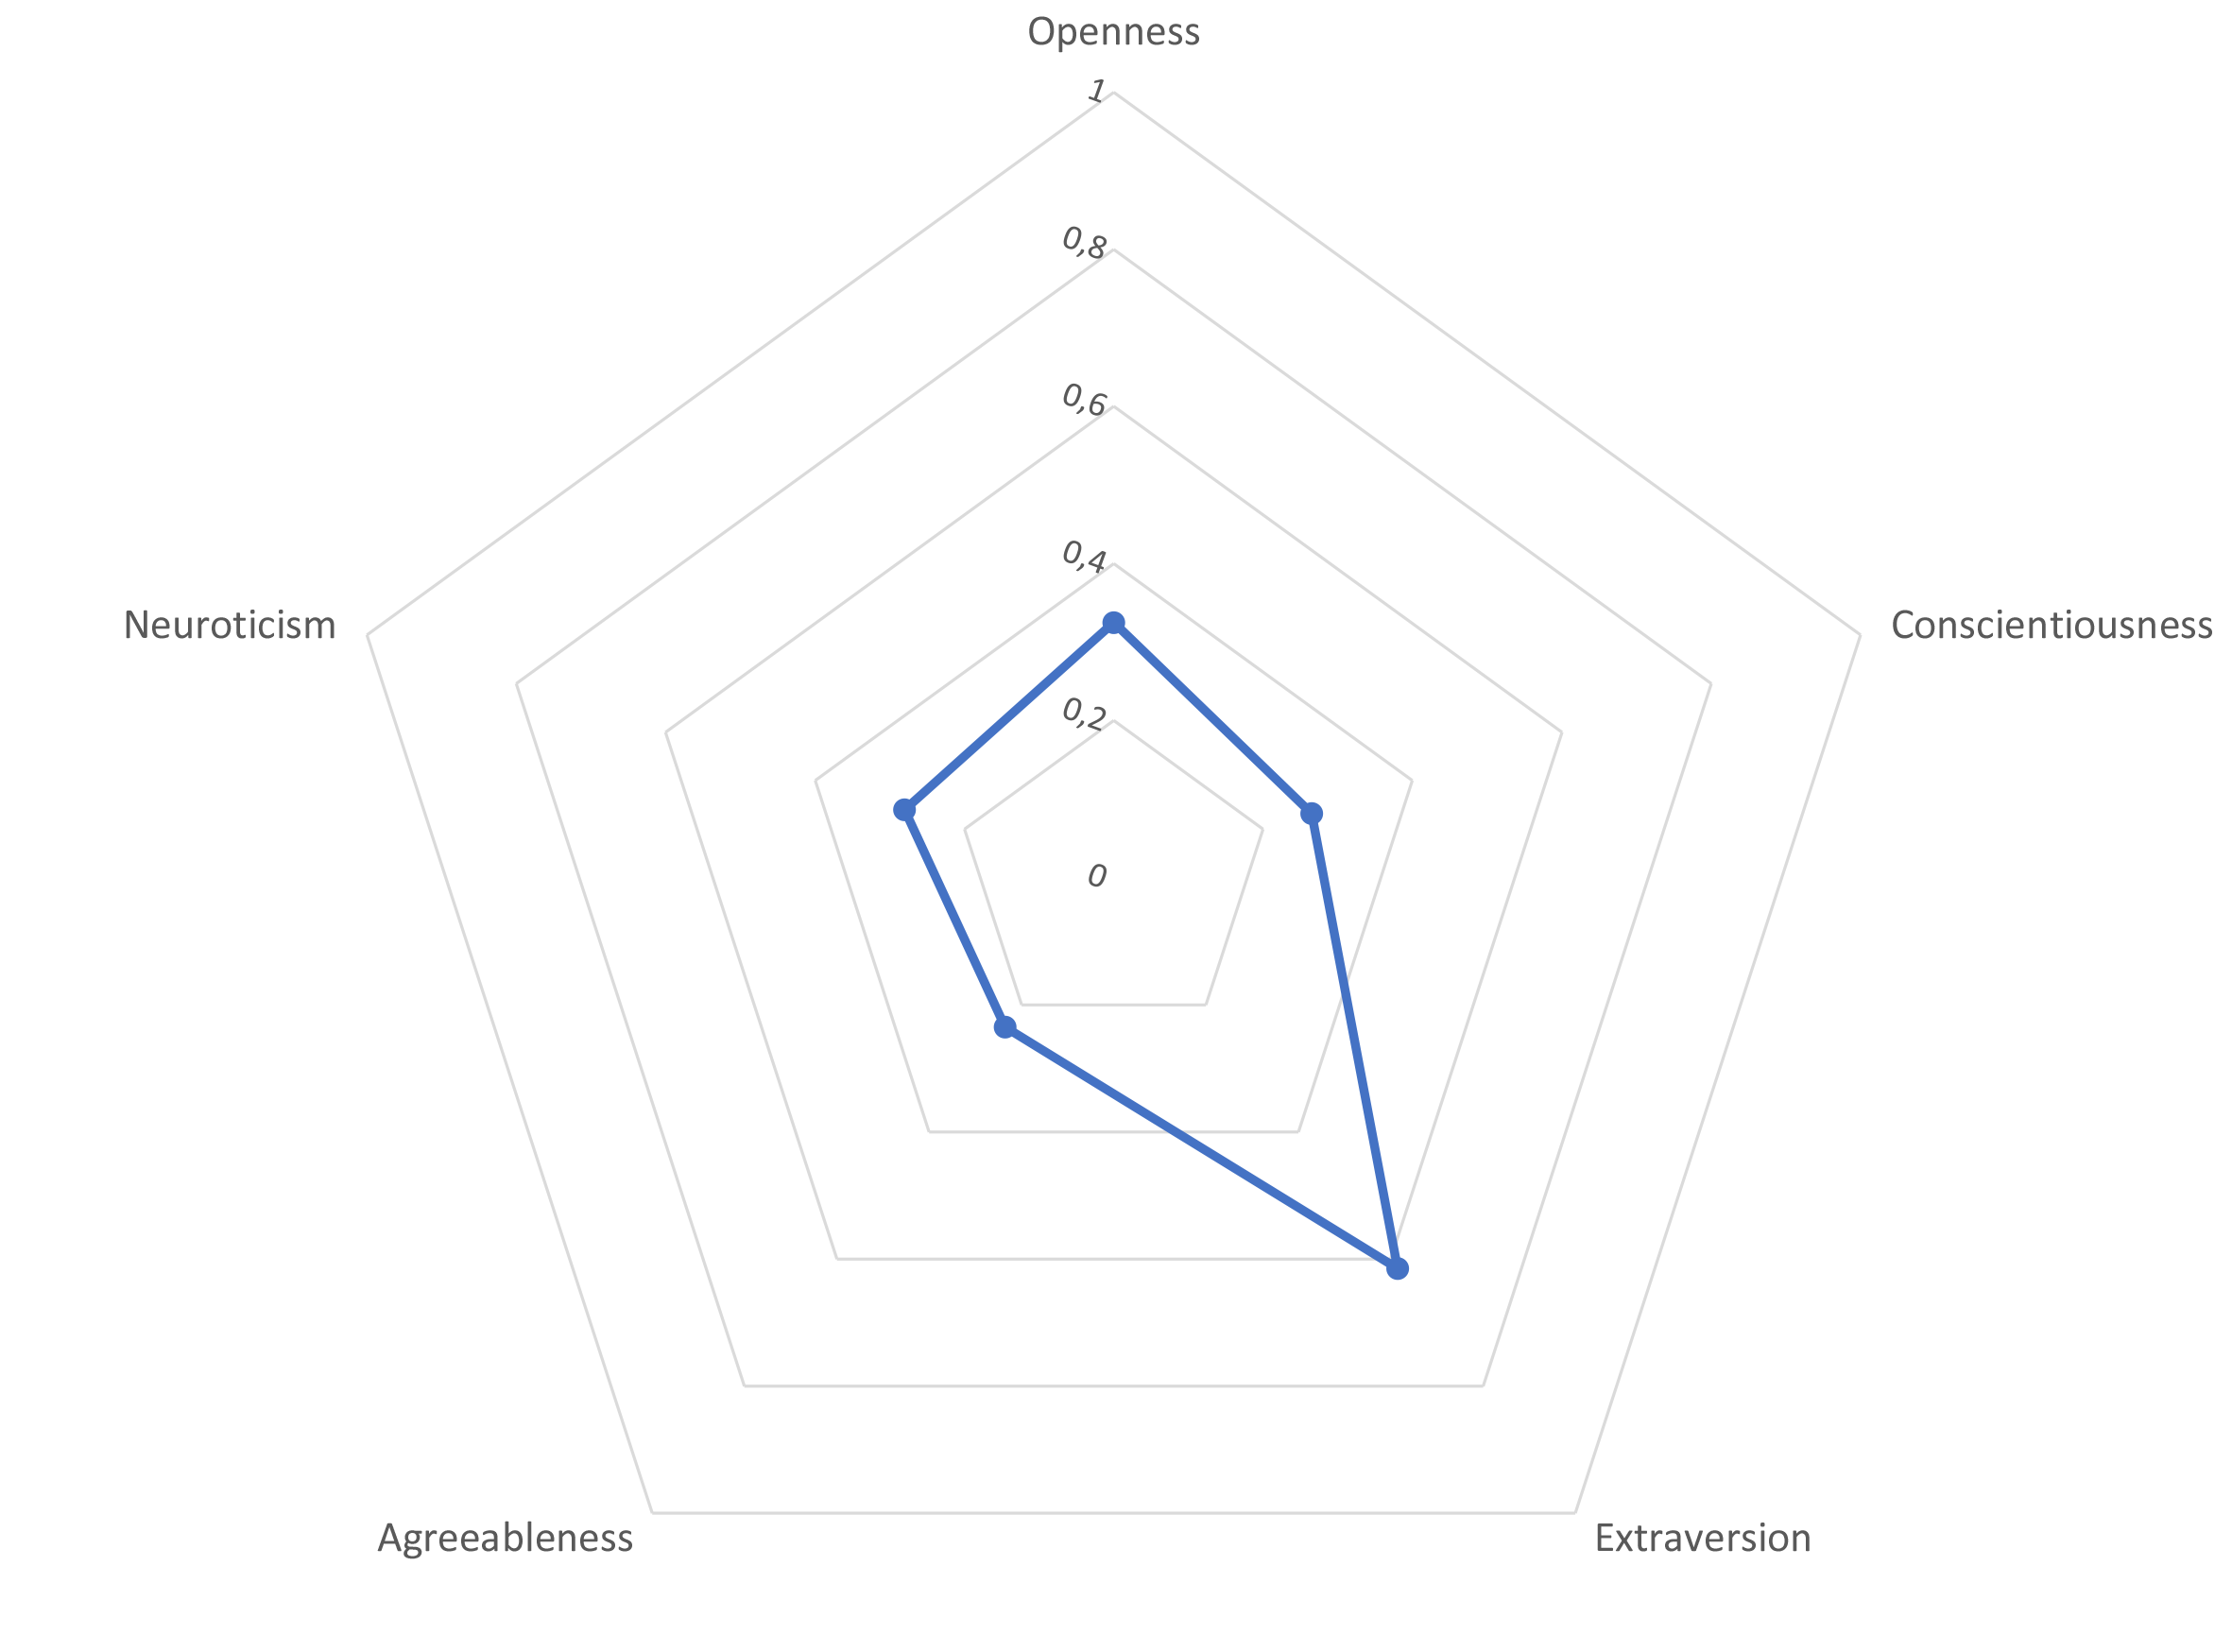
\includegraphics[scale=0.35]{figure/graph4_sanguine}}
    \subfloat[Phlegmatic graph][Phlegmatic]{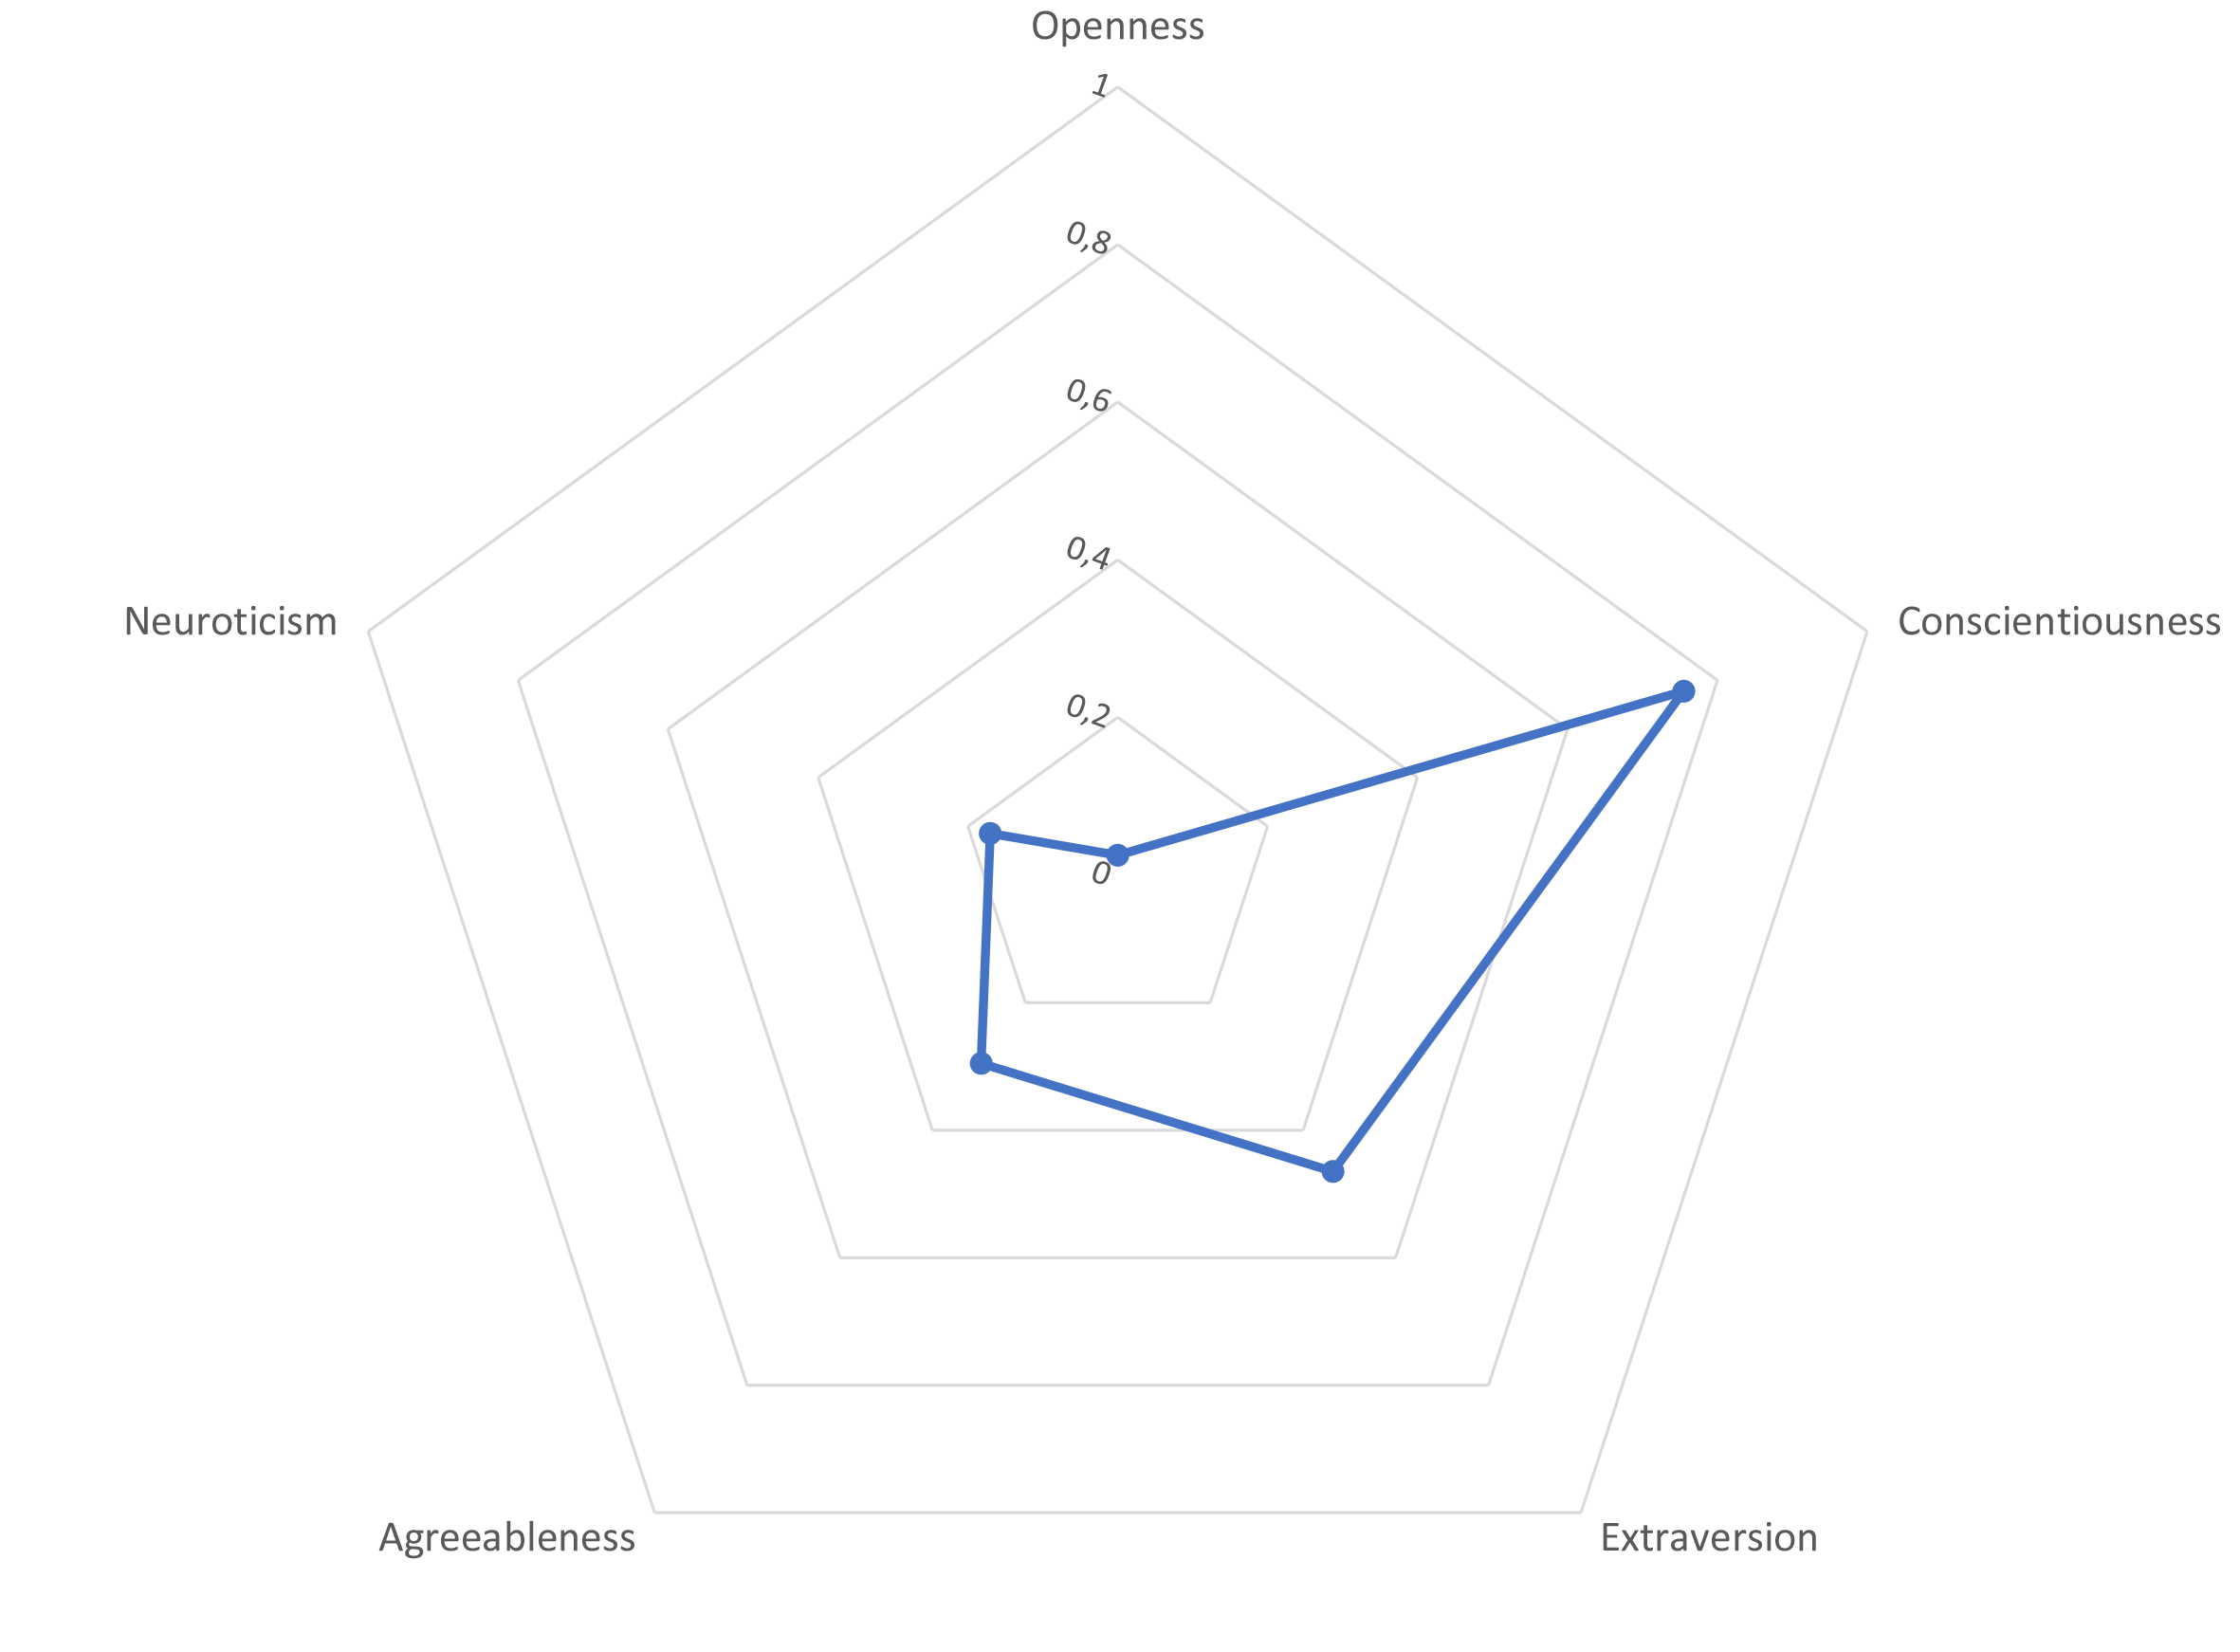
\includegraphics[scale=0.35]{figure/graph3_phlegmatic}}
  \captionsetup{justification=centering}
    \caption{The four graphs representing the correlation between each of the Four Temperaments and the factors that define the Big 5 model.}
    \label{fig:4t-big5}
\end{figure}
\section{Data Collection}\label{subsec:dataresults}
Trying to counterbalance the lack of user-friendliness of the Tiltyard server, and the time-consumption of some of the games that have been chosen, the data collection process has been ongoing from the beginning of this project to the very last weeks. However, once the data training had started, only the collection of Skirmish games was allowed, namely the matches required for the evaluation process.\\
Overall, data has been collected for 84 matches, in 46 different games, with 17 different users. The games involving two human players have been considered as two different matches for the genetic algorithm training, being associated to two different personalities and gaming styles. All users had different background and board games experience, and the most experienced players have been asked to try multiple games changing their playing style, trying to associate it to each of the different procedural personæ. Thanks to this, although the amount of games collected has been lower than expected, the distribution of games and personalities has been tendentially homogeneous in both personality and games distribution, as it can be seen from table \ref{tab:datac}.\\
\begin{table}[h]
    \caption{Summary of the games collected and the personality the users self-associated to themselves.}
    \centering
    \scriptsize
	\begin{tabular}{|c|c|c|c|c||c|}
    	\hline
					& Checkers & Skirmish & Connect Four & Nine Board Tic-Tac-Toe & Tot. \\
        \hline
        Melancholic & 1  & 3 & 4  & 17 & 25 \\
        \hline
        Choleric	& 5  & 1 & 8  & 8  & 22 \\
        \hline
        Phlegmatic	& 0  & 1 & 3  & 9  & 13 \\
        \hline
        Sanguine	& 4  & 3 & 11 & 6  & 23 \\
        \hline \hline
        Tot.		& 10 & 8 & 26 & 40 & 84 \\
        \hline
	\end{tabular}
    \label{tab:datac}
\end{table}
\noindent In the questionnaire given to the users, aside their own personality, they also have been asked to specify which personality they were perceiving from their opponent. Considering some bias toward the Phlegmatic personality due to Tiltyard's slow response, we can generally see a tendency in associating the opponents to the Melancholic and the Phlegmatic personalities, while the self-definition results in a more homogeneous spread. In table \ref{tab:datacpp} can be seen the summary of the perceived personalities of the opponents.\\
\begin{table}[h]
    \caption{Summary of the games collected and the perceived personality the users associated to their opponents.}
    \centering
    \scriptsize
	\begin{tabular}{|c|c|c|c|c||c|}
    	\hline
					& Checkers & Skirmish & Connect Four & Nine Board Tic-Tac-Toe & Tot. \\
        \hline
        Melancholic & 5  & 3 & 5  & 22 & 35 \\
        \hline
        Choleric	& 1  & 2 & 6  & 11  & 20 \\
        \hline
        Phlegmatic	& 4  & 2 & 10  & 5  & 20 \\
        \hline
        Sanguine	& 0  & 1 & 5 & 2  & 8 \\
        \hline \hline
        Tot.		& 10 & 8 & 26 & 40 & 84 \\
        \hline
	\end{tabular}
    \label{tab:datacpp}
\end{table}
As mentioned above, the Phlegmatic's numbers might be slightly skewed, inferring some false positive when the Tiltyard server was being unresponsive, and some false negative when the users realised that the long turns might have been caused by the system (ignoring completely - in such case - the possible phlegmatic tendency of the opponent). However, considering that a good part of our testers were in communication with each other - either in the same room, or in the IRC channel set up for them - we still think that, overall, the collected results could be meaningful. Nonetheless, this is the reason why only the self-described personality is taken into consideration for the training of our genetic algorithm.
It is interesting to see that among the 84 matches collected, in 16 of them (almost $20\%$) either of the players perceived the personality that was self defined by the opponent. The distribution of the success in matching the opponents personality can be found in table \ref{tab:matching}.
\begin{table}[h]
    \caption{Summary of the games where the users recognized successfully the opponent's personality.}
    \centering
    \scriptsize
	\begin{tabular}{|c|c|c|c|c||c|}
    	\hline
					& Checkers & Skirmish & Connect Four & Nine Board Tic-Tac-Toe & Tot. \\
        \hline
        Melancholic & 1 & 0 & 0 & 5  & 7 \\
        \hline
        Choleric	& 0 & 0 & 1 & 3  & 4 \\
        \hline
        Phlegmatic	& 0 & 1 & 2 & 1  & 3 \\
        \hline
        Sanguine	& 0 & 0 & 1 & 1  & 2 \\
        \hline \hline
        Tot.		& 1 & 1 & 4 & 10 & 16 \\
        \hline
	\end{tabular}
    \label{tab:matching}
\end{table}
Checkers and Skirmish were unknown games to most of the users before participating in the data collection, and that would excuse the inability to recognize any pattern, or strategy, in the opponent's game. Whilst Nine Boards Tic-Tac-Toe was a new game as well, the simple correlation to basic Tic-Tac-Toe, could have improved the process of following the gameplay. On the other hand, it can be assumed that the Melancholic type has been the most recognized as it might be easier to understand, by the end of the game, if the opponent has had a long term strategy ongoing during the whole match. 
\section{Genetic Algorithm}\label{sec:gares}
The Genetic Algorhtm has been executed a few times, over different sized sets of data, and the first thing to be noticed it  that the general fitness was much lower than it hoped for, causing the terminating test depending on acceptable fitness value $f_a=0.9$, to be unused. Only stagnancy of the individuals was then defining whether the algorithm would have terminated or not.\\


It has been mentioned in \ref{sec:ga} that a few test runs have been carried out in order to define which values to assign to the probabilities of crossover and mutation, $p_c$ and $p_{mut}$, and creep rate $C_r$. Those values have been tuned after several tests over the Phlegmatic's batch of games, which was the quickest to execute. The execution time of each block of games depended heavily on the games played, rather than on the parameters selection themselves. It is found that the Choleric and Sanguine batch, containing a higher number of Checkers games, are noticeably slower than the Phlegmatic group. In figure \ref{fig:runtimes} it can be seen how the Phlegmatic individuals have running time on the scale of $10^4ms$, while Choleric and Sanguine have it on the scale of $10^6ms$. The graphs also show how much impact the different parameters have on the execution times, which is generally consistent in the same personality data group, if we exclude a few noticeable peeks that reduce in number and intensity with the increasing of the generations. 
\begin{figure}[h]
\centering
    \subfloat[Choleric graph][Choleric] {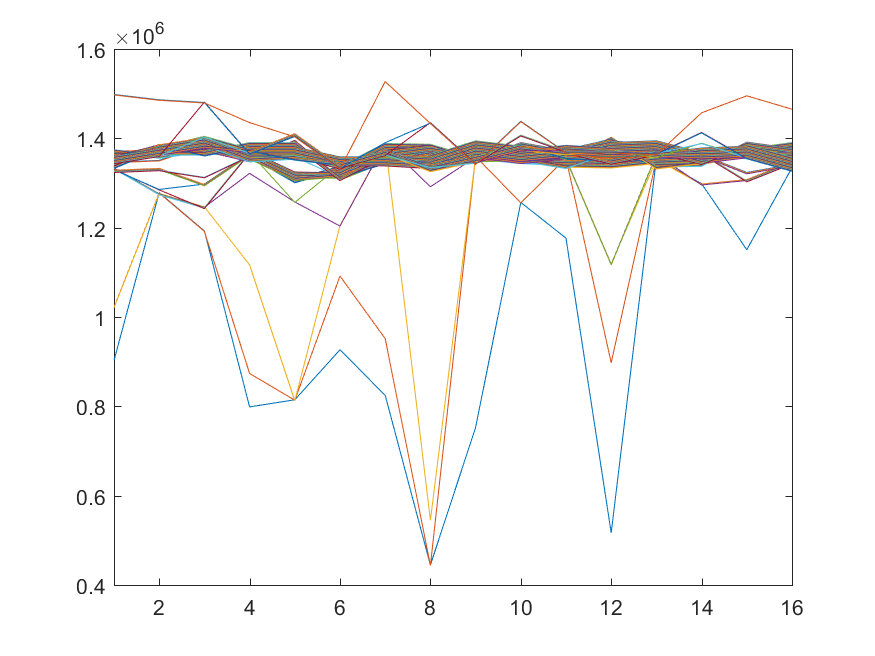
\includegraphics[scale=0.45]{figure/runtimeCh}}
    \subfloat[Melancholic graph][Melancholic]{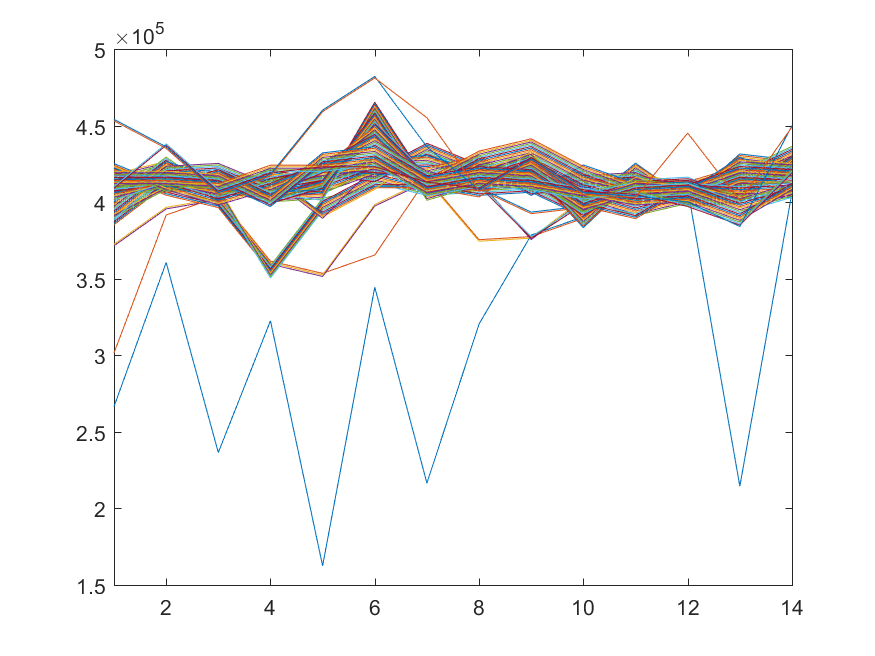
\includegraphics[scale=0.45]{figure/runtimeMe}}
    \qquad
    \subfloat[Sanguine graph][Sanguine]{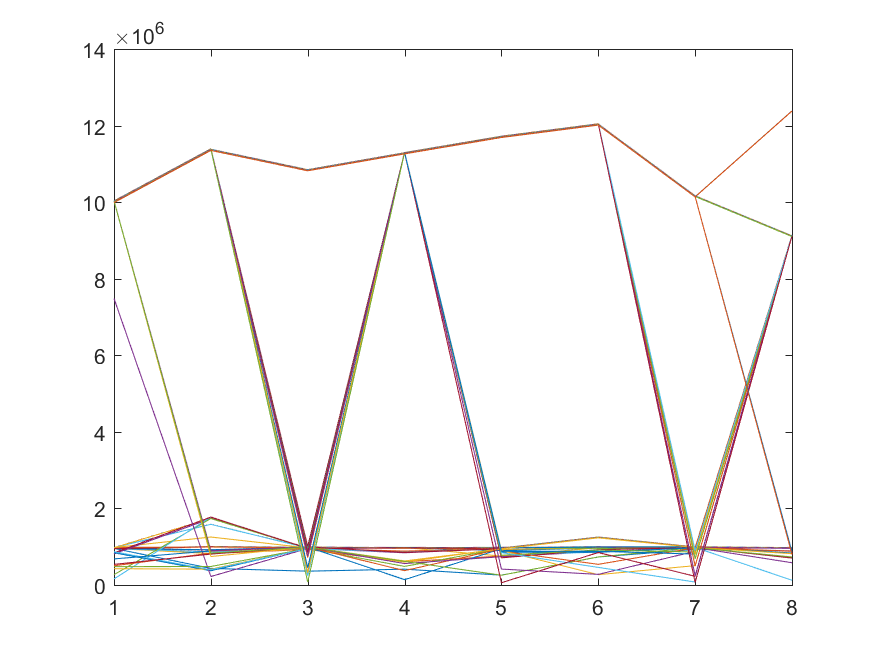
\includegraphics[scale=0.45]{figure/runtimeSa}}
    \subfloat[Phlegmatic graph][Phlegmatic]{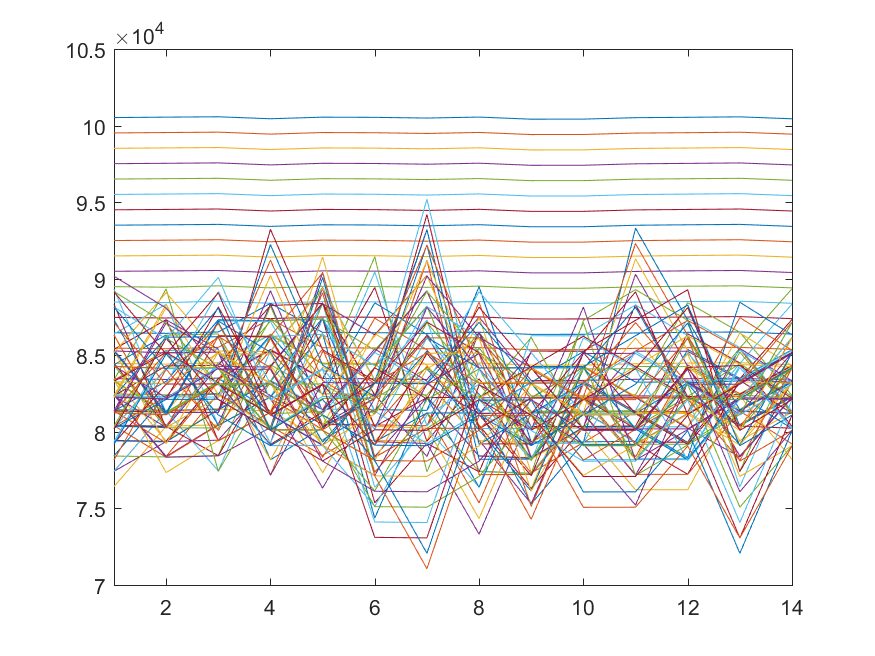
\includegraphics[scale=0.45]{figure/runtimePh}}
  \captionsetup{justification=centering}
    \caption{The four graphs represent the running times (in ms) for all the individuals in each generation, on y and x axis respectively.}
    \label{fig:runtimes}
\end{figure}

\subsection{Results Overview}
In Appendix \ref{sec:genegraphs} can be found the plots of the single individuals over three runs of the genetic algorithm. Each page contains the plots of the single genes, for each individual in each generation. Of those three runs, the first one has a different set of "algorithm" values $p_c$, $p_{mut}$, and $C_r$ than the ones described in section \ref{sec:ga}. Specifically, the first run adopts $p_c=0.8$, $p_{mut}=0.015$, and $C_r=0.2$. The first thing to be noticed from those plots is the number of generations. Although different "algorithm" values have been tested over a set of the data in order to maximise the number of generations - as mentioned earlier -, after the first tests, the results have become inconsistent. Several runs took long to stagnate (over 40 generations), whilst took other only few (8, for example). It has finally been decided to keep the same set of values, given the unpredictability of the number of evolutions.\\


It is to be noticed that different personalities tend to different values for the same gene. However, it is also to be pointed out that different runs aim at different results as well. That can be excused as the optimal individual that is picked does not look the same for each execution, leading to slightly different values combinations. Looking in more detail to some of the graphs in Appendix \ref{sec:genegraphs} it can be said that, when, for the each personality, different executions return very diverse values for the same parameter. What it means is that each parameter alone is not really relevant in the actions-matching for the personality in exam, as for example, the \emph{ChargeDefault} (see figure \ref{fig:phleChargeDef}). This statement can be clarified looking at figure \ref{fig:chargcorrl}. 
\begin{figure}[H]
\centering
    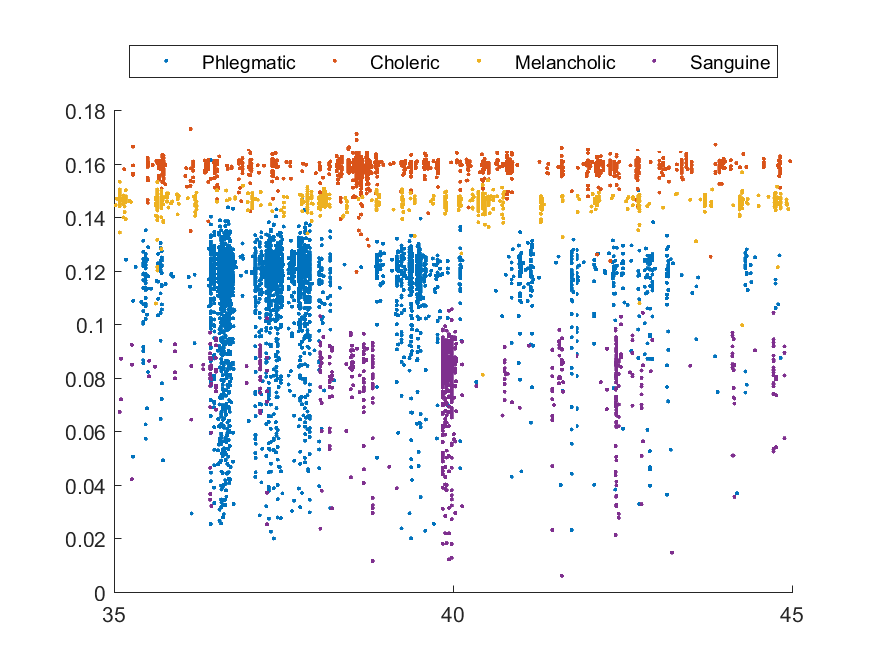
\includegraphics[scale=0.4]{figure/indfit/chargedeffit}
  \captionsetup{justification=centering}
    \caption{Correlation between specific Charge Default and fitness.}
    \label{fig:chargcorrl}
\end{figure}
It can be seen that each genes clusters around some specific values, however, not in a meaningful distribution. Further correlations need to be investigated, to understand which combination of parameters is indeed useful to influence the agent's game, and which are not.
\begin{figure}[ht!]	
\centering
    \subfloat[][Phlegmatic - I run]{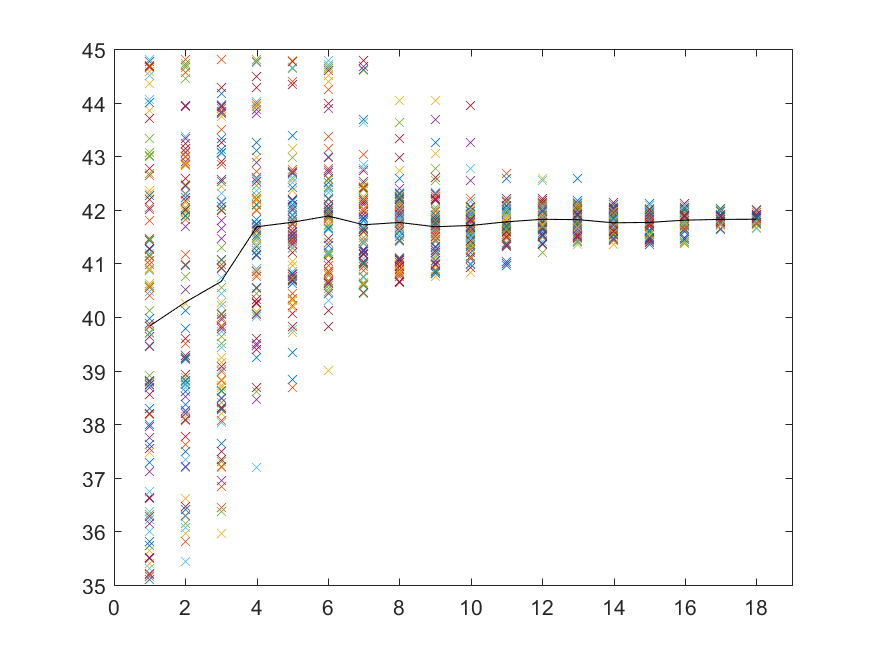
\includegraphics[scale=0.34]{figure/graphs1run/chargedefP}}
    \subfloat[][Phlegmatic - II run]{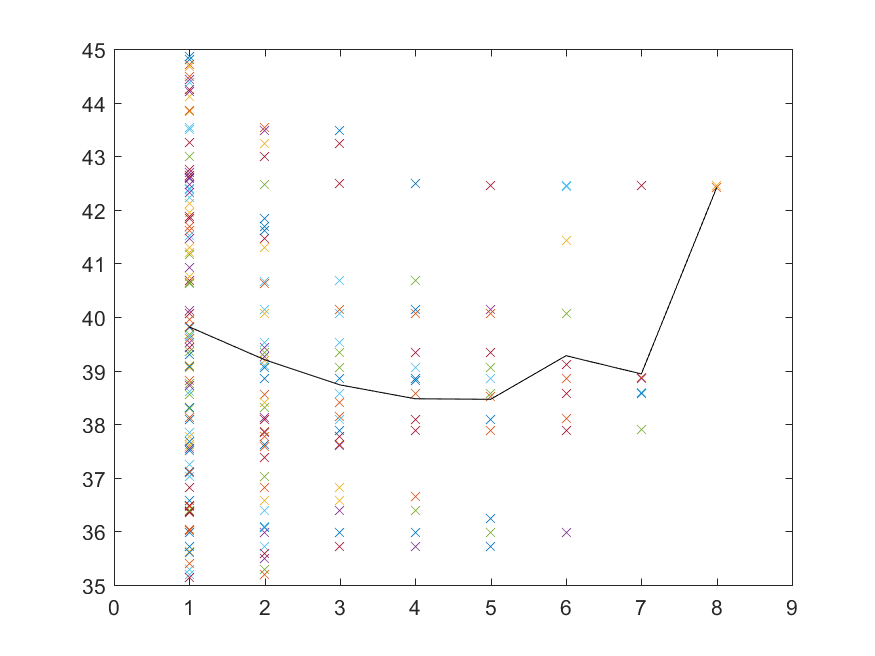
\includegraphics[scale=0.34]{figure/graphs2run/chargedefP}}
    \subfloat[][Phlegmatic - III run]{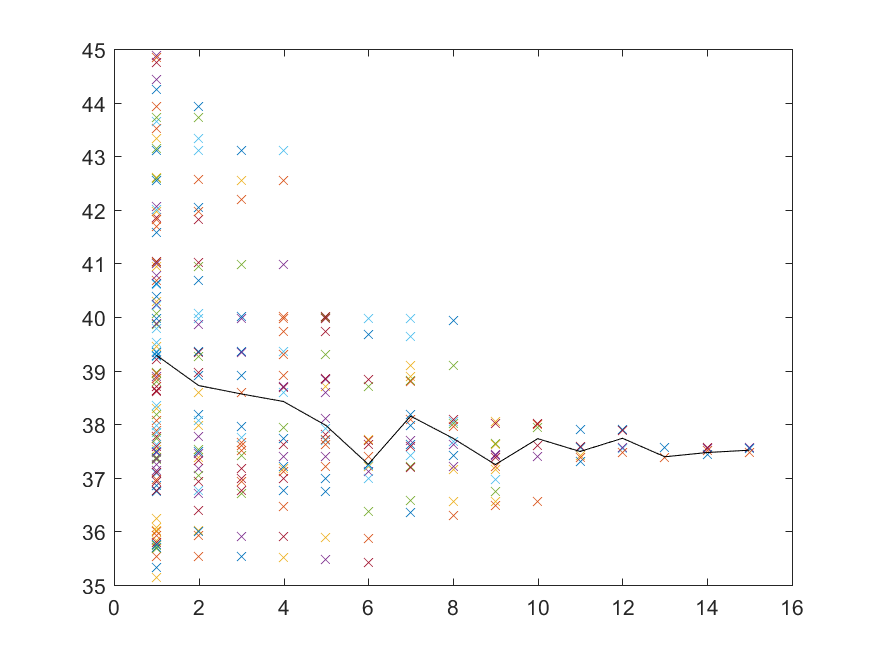
\includegraphics[scale=0.34]{figure/graphs3run/chargedefP}}
  \captionsetup{justification=centering}
  \caption{Charge Default gene for Phlegmatic personality.}
  \label{fig:phleChargeDef}
\end{figure}
It can also be noted from figure \ref{fig:explfact} that the \emph{Exploration Factor} gene seems to tend to the same value independently of the personality.\\
From the \emph{horizon} graphs in figure \ref{fig:horizon} it can be seen that the Melancholic type has generally a higher valued outcome, as it would be expected, being it the personality with the higher correlation to game strategy. In the same way, the parameter $NiceThreshold$ seems to generally be higher for Phlegmatic and Sanguine, and our model confirms them to be the two personalities with lower competitiveness. Figure \ref{fig:nicethresR} collects the results for the gene, after the third run.
\begin{figure}[ht!]
\centering
	\subfloat[][Choleric - III run] {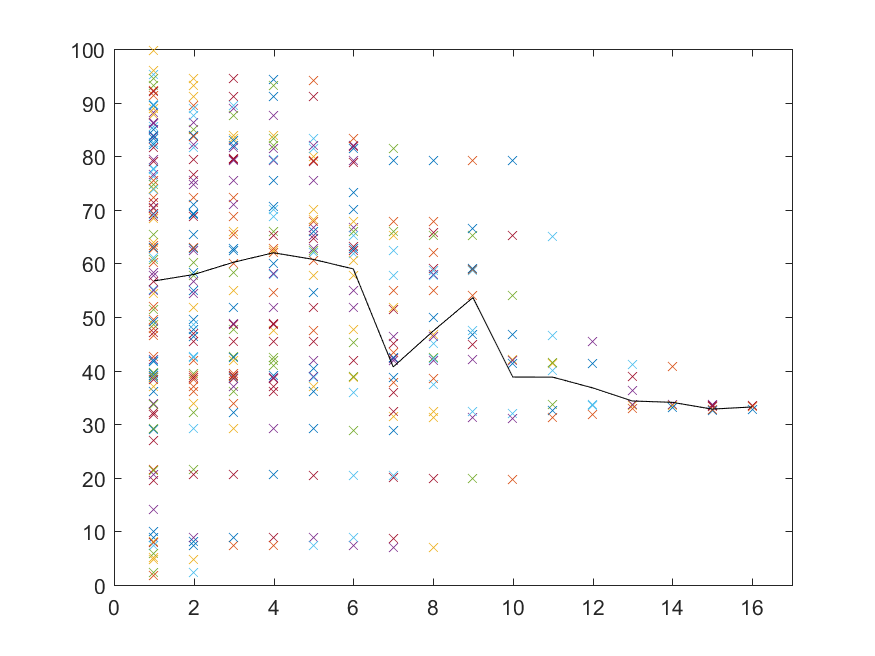
\includegraphics[scale=0.35]{figure/graphs3run/nicethresC}}
    \quad
    \subfloat[][Melancholic - III run]{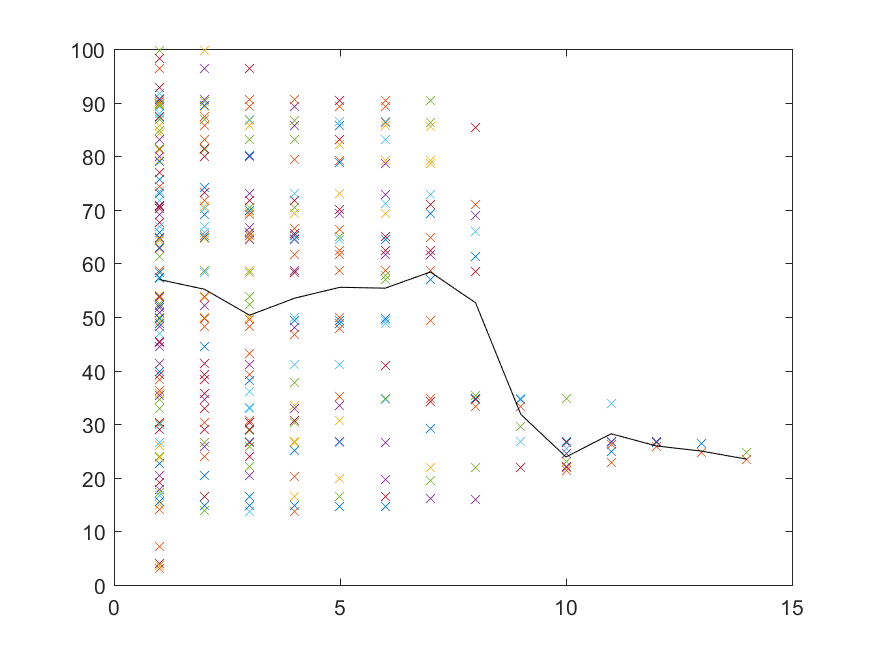
\includegraphics[scale=0.35]{figure/graphs3run/nicethresM}}
    \quad
    \subfloat[][Sanguine - III run]{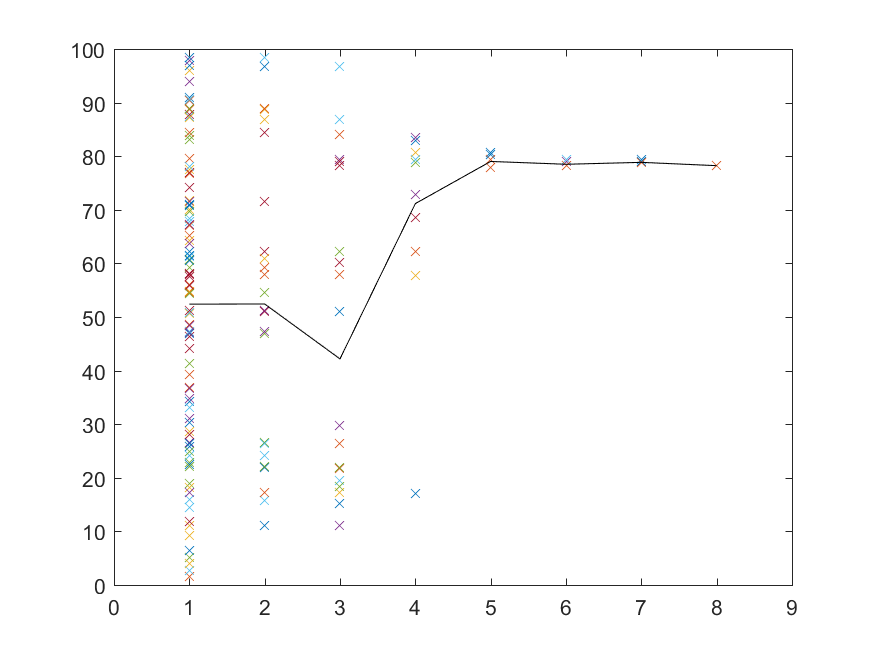
\includegraphics[scale=0.35]{figure/graphs3run/nicethresS}}
	\quad
    \subfloat[][Phlegmatic - III run]{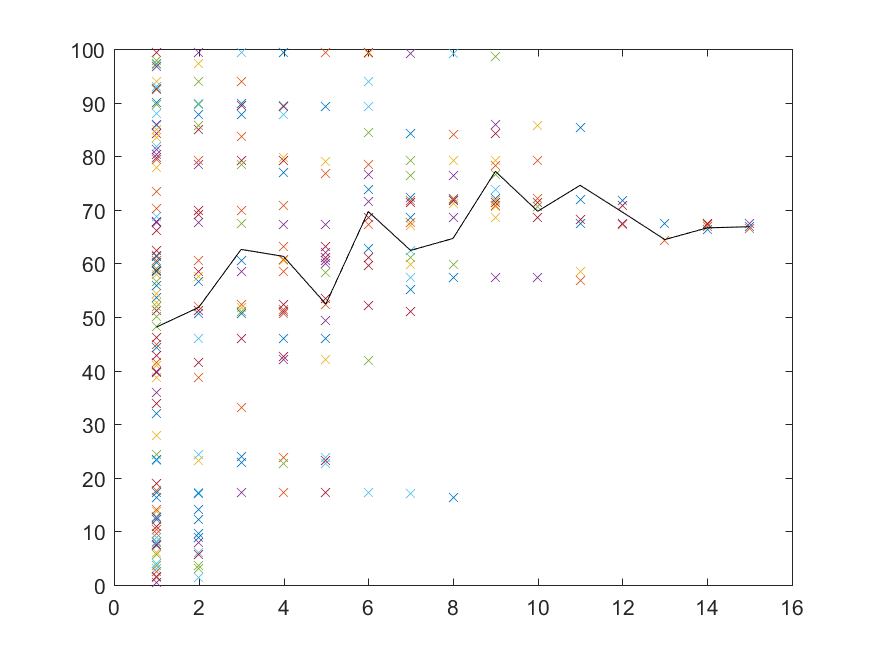
\includegraphics[scale=0.35]{figure/graphs3run/nicethresP}}
  \captionsetup{justification=centering}
    \caption{Nice Threshold gene's results of the III run.}
    \label{fig:nicethresR}
\end{figure}
Contrarily to our expectations, the \emph{RandomError} variable tends to a probability $P(RandomError)=0.5$, or higher in some cases (see figure \ref{fig:randomerrorR} for a clearer picture). We recall that this parameter controls the probability of picking a random move instead of the one suggested by the search. This means that half of the actions the MCTS outputs are aleatory, and that influences the fitness of the individuals, decreasing the helpfulness of elitism in keeping the individual with the highest fitness for the following generations.
\begin{figure}[h]
\centering
	\subfloat[][Choleric - III run] {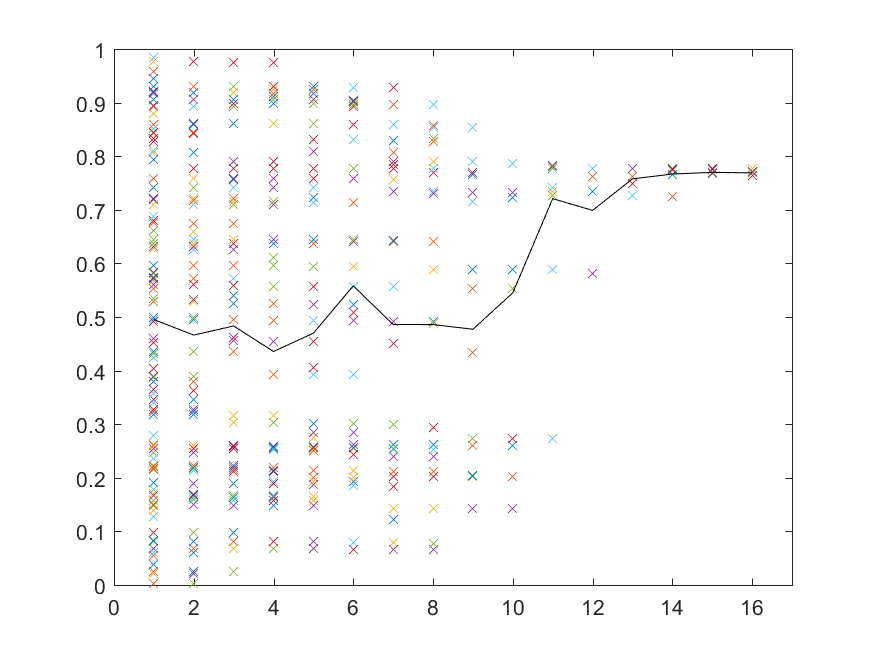
\includegraphics[scale=0.35]{figure/graphs3run/randomerrorC}}
    \quad
    \subfloat[][Melancholic - III run]{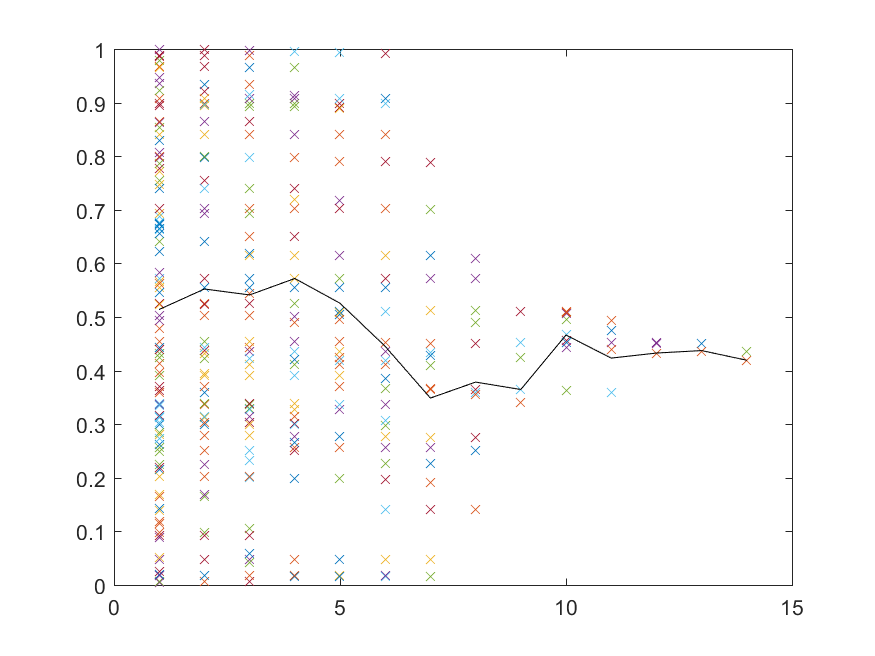
\includegraphics[scale=0.35]{figure/graphs3run/randomerrorM}}
     \quad
    \subfloat[][Sanguine - III run]{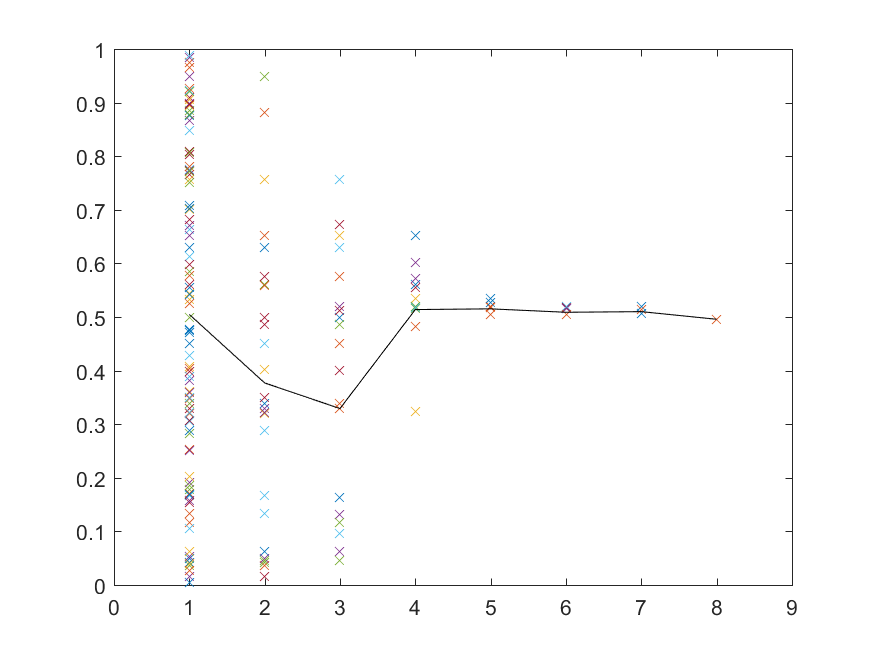
\includegraphics[scale=0.35]{figure/graphs3run/randomerrorS}}
	\quad
    \subfloat[][Phlegmatic - III run]{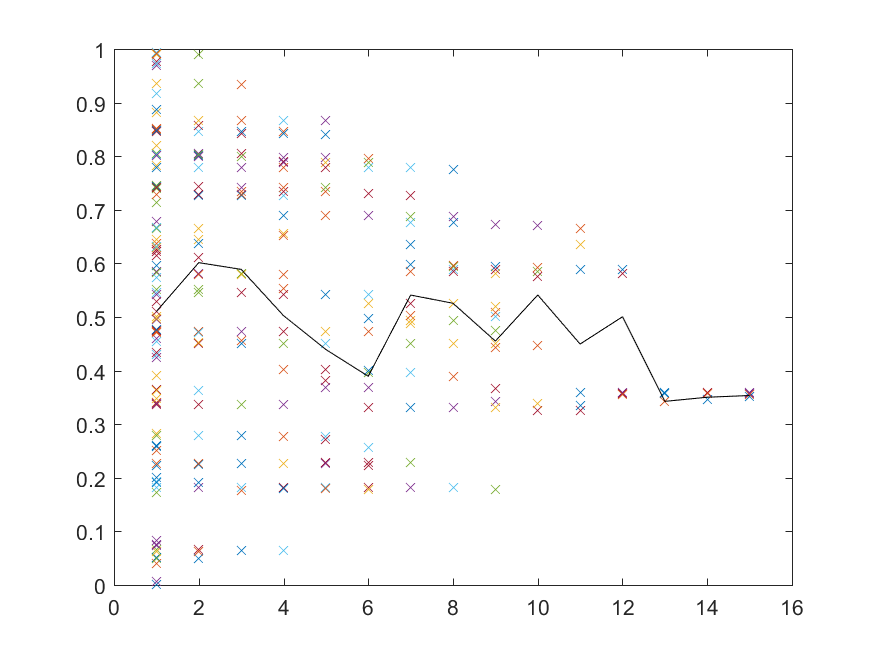
\includegraphics[scale=0.35]{figure/graphs3run/randomerrorP}}
  \captionsetup{justification=centering}
    \caption{Random Error gene's results of the III run.}
    \label{fig:randomerrorR}
\end{figure}
\subsection{Fittest Individuals}
After a few executions of the Genetic Algorithm, the fittest individuals for each of them have been picked to feed the evaluation process. The values are collected in table \ref{tab:fittest}. The Genetic Algorithm returns all doubles; the parameters are casted to the supposed type when plugged into the MCTS algorithm. The table aforementioned contains values that are partially already rounded (the ones with type \emph{long}, to be exact), while the floating point ones are rounded to the third decimal place.
\begin{table}[h]
	\caption{Fittest individuals picked for evaluation.}
    \centering
    \scriptsize
    \begin{tabular}{|c|c|c|c|c|}
    \hline
    Parameter & Phlegmatic & Sanguine & Choleric & Melancholic \\
        \hline
    epsilon & 0.264 & 0.507 & 0.435 & 0.045\\
        \hline
    rave & 2328 & 2744 & 4102 & 832\\
        \hline
    grave & 65 & 71 & 84 & 55\\
        \hline
    chargeDiscount &  0.937 & 0.947 & 0.985 & 0.930\\ 
        \hline
    treeDiscount & 0.952 & 0.943 & 0.972 & 0.969\\
        \hline
    aggression & 1.259 & 1.533 & 1.796 & 2.622\\ 
        \hline
    defensiveness & 1.161 & 1.878 & 0.208 & 0.725\\ 
        \hline
    chargeDepth & 53 & 54 & 47 & 61\\ 
        \hline
    horizon & 12 & 12 & 11 & 19\\
        \hline
    randErr & 0.503 & 0.451 & 0.398 & 0.380\\
        \hline
    chargeDefault & 41.768 & 40.014 & 39.984 & 35.782\\
        \hline
    explorationFactor & 68 & 81 & 71 & 105\\ 
        \hline
    niceThreshold & 33.903 & 55.308 & 24.593 & 12.885\\
        \hline
    \end{tabular}
    \label{tab:fittest}
\end{table}
In figure \ref{fig:fitnessfunc} can be seen the evolution of the fitness function, generation after generation. The red line represents the fitness of the fittest individual, calculated with equation (\ref{eq:fitnessfunc}); the blue line represents the average fitness of the individuals in that generation, while the blue errorbars are the standard deviation. Lastly, the black line represents the probability of picking a random move, referred here as "random-fitness". It was calculated as the geometric mean over all the matches of the probability $P(AnyMove)=\frac{1}{AvailableMoves}$ for each state. Considering that the MCTS is run always from the same state, it is expected that the probability $P(AnyMove)$ is constant throughout the generations. The optimal outcome would have been having the fitness of the fittest individual topping the random-fitness, but that is not true for most of the personalities. Figure \ref{fig:fitnessfunc} presents data from two different runs, as it is expected to be equally meaningful, the presented data has been chosen only on the basis of being clearer, although the results between executions are slightly different, they are equivalent nonetheless. 
\begin{figure}[ht!]
\centering
	\subfloat[][Choleric - III run] {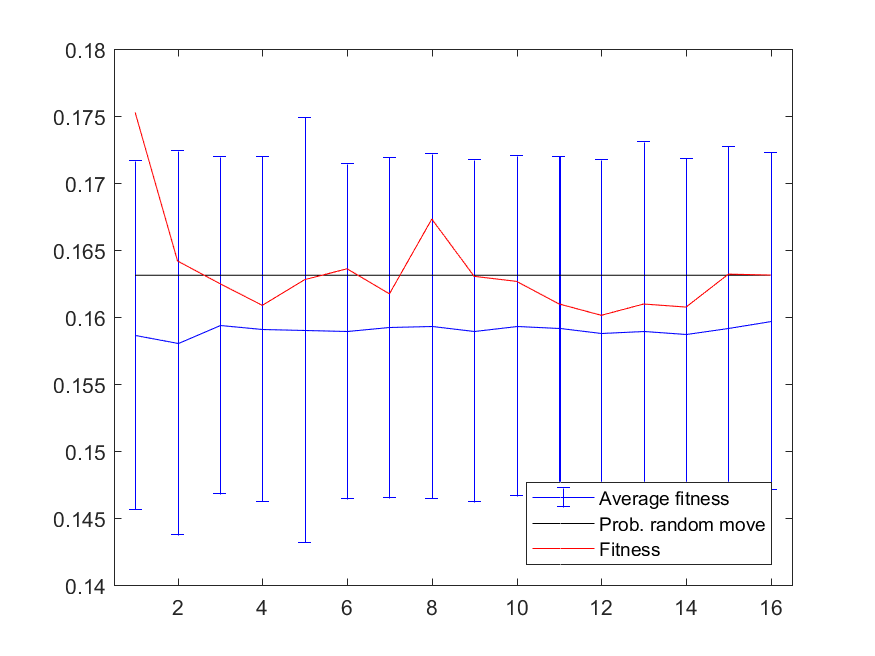
\includegraphics[scale=0.45]{figure/randCh}}
    \quad
    \subfloat[][Melancholic - IV run]{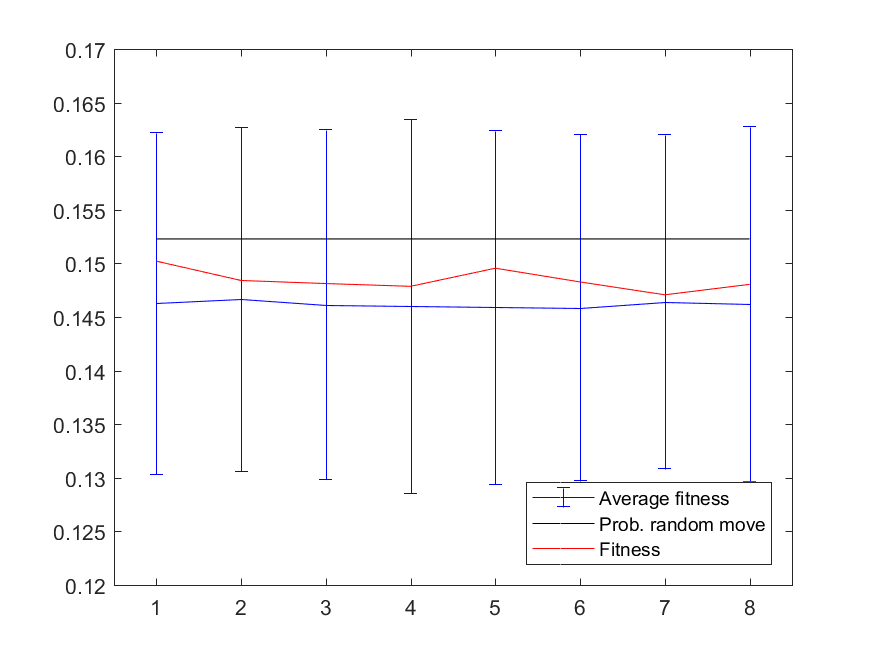
\includegraphics[scale=0.45]{figure/randMe}}
     \quad
    \subfloat[][Sanguine - IV run]{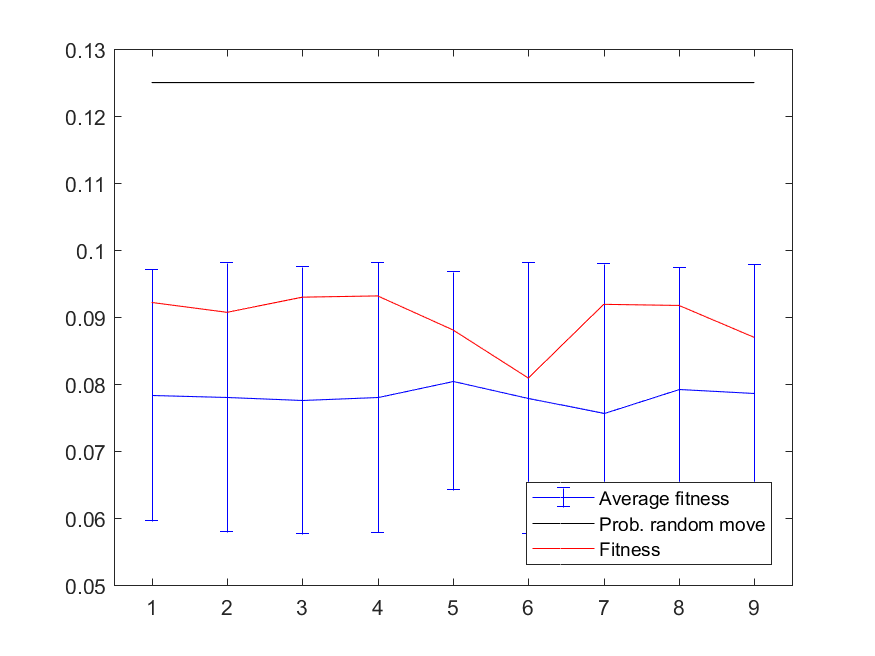
\includegraphics[scale=0.45]{figure/randSa}}
	\quad
    \subfloat[][Phlegmatic - III run]{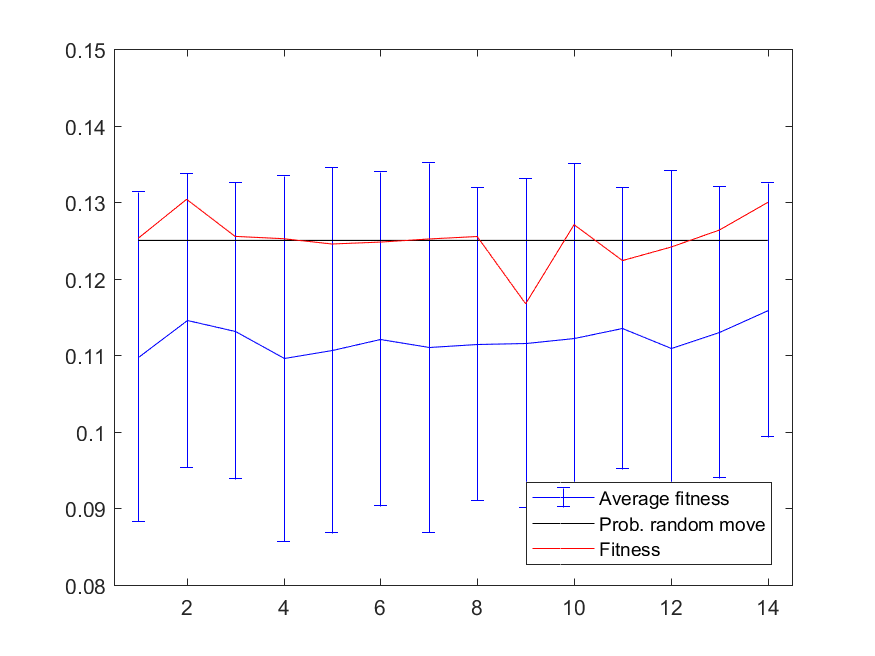
\includegraphics[scale=0.45]{figure/randPh}}
  \captionsetup{justification=centering}
    \caption{Fitness evolution throughout the generations, for each personality.}
    \label{fig:fitnessfunc}
\end{figure}
It is to be noted that, while the fittest individual is -averagely- not much better than only picking random moves at each turn, it is still above the average fitness among the individuals in the same generation, as expected.\\
For completeness, it is to be pointed out that only at report composing time it has been found a discrepancy between the geometric mean calculated by MATLAB (plotted in the graphs), and the one returned in the genetic algorithm logs. This is indeed a problem to be fixed, but considered the demanding computation required by the algorithm, it has been decided that this difference is irrelevant for the conclusions to be drawn.

\section{Results Game Play}\label{sec:reeval}
Among the games collected, only the Skirmish ones are used for evaluation purposes. Together with the skimming over the games recovered from the Tiltyard's bulks, it lead us to a total of 8 Skirmish games from the data collection and 54 games from the archives, divided in 22 Connect Four, 24 Nine Boards Tic-Tac-Toe, and 6 Checkers matches.
The evaluation algorithm has been running with the fittest individuals outputted by the genetic algorithm (see table \ref{tab:fittest}), and a set of random ones. The results are described below, while a selection of the gameplays' graphs can be found in appendix \ref{sec:genegraphs}.
\subsection{Skirmish Games with Fittest Individuals}
The first evaluation process has taken the fittest individuals resulting from the genetic algorithm. 
\begin{figure}[ht!]
\centering
	\subfloat[][Choleric] {\includegraphics[scale=0.45]{figure/eval/Skirmish/evalMatchskirCh1}}
    \quad
    \subfloat[][Melancholic]{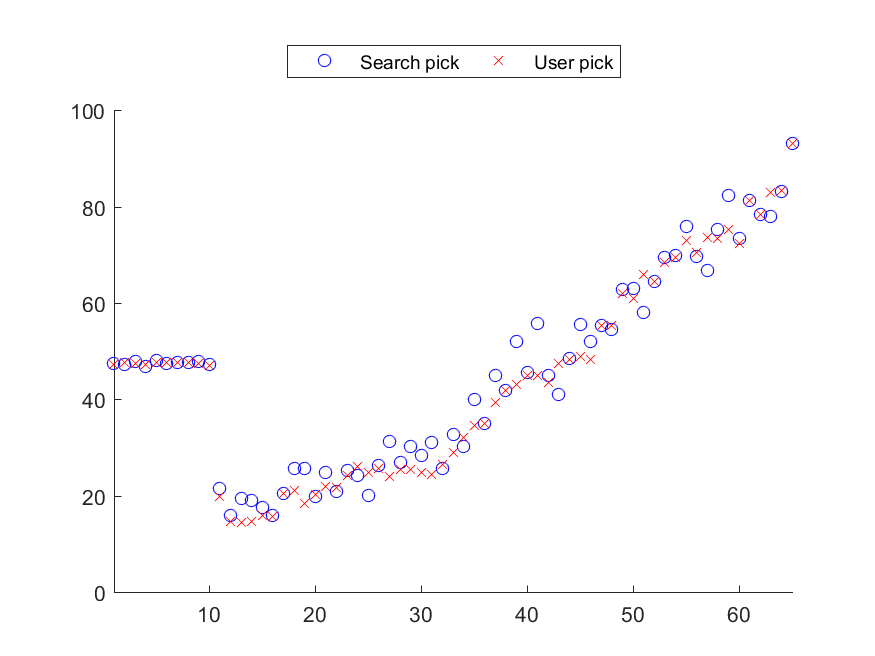
\includegraphics[scale=0.45]{figure/eval/Skirmish/evalMatchskirMe3}}
     \quad
    \subfloat[][Sanguine]{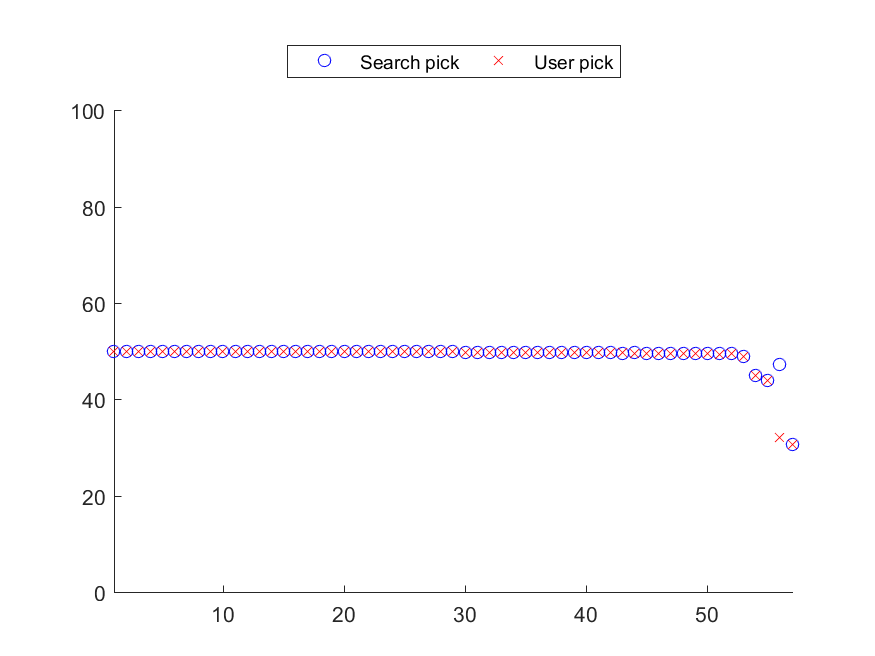
\includegraphics[scale=0.45]{figure/eval/Skirmish/evalMatchskirSa2}}
	\quad
    \subfloat[][Phlegmatic]{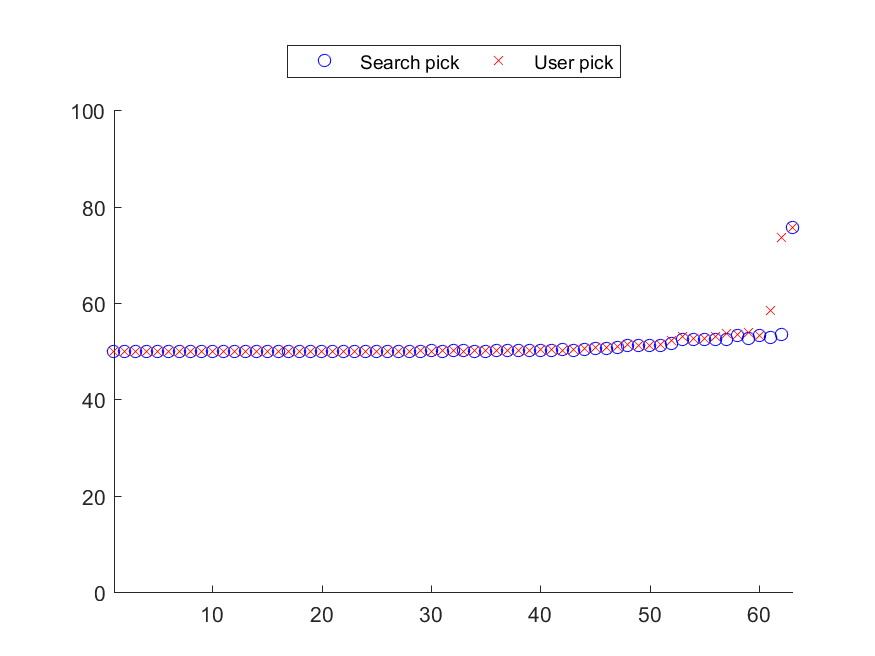
\includegraphics[scale=0.45]{figure/eval/Skirmish/evalMatchskirPh1}}
  \captionsetup{justification=centering}
    \caption{Evaluation of Skirmish matches.}
    \label{fig:skirmishE}
\end{figure}
Figure \ref{fig:skirmishE} shows the results of one Skirmish game for each personality, played with the "correct" parameters outputted by the GA. Although the logs confirm that search moves are not actually the same as the user's, figure \ref{fig:skirmishE} shows that the selected moves had an extremely similar QValue. It is necessary to point out that Skirmish is a game with a lot of legal moves at each state, averaging then the values of all of them. Table \ref{tab:cholski} contains the list of last moves in the Choleric game, to show that the actions selected are, as matter of fact, different, but essentially with the same weight.
\begin{table}[H]
	\caption{Last moves in the Choleric-Skirmish game.}
    \centering
    \scriptsize
    \begin{tabular}{|c|c|c|c|c|}
    \hline
    Search Action & QValue & User Action & QValue \\
        \hline
        {[( move 1 5 4 8 ), noop]} & 49.495 & {[( move 6 7 4 5 ), noop]} & 49.720\\
        {[noop, ( move 5 4 6 6 )]} & 49.791 & {[noop, ( move 5 4 4 6 )]} & 49.773\\
        {[( move 4 5 3 4 ), noop]} & 49.953 & {[( move 3 8 4 7 ), noop]} & 49.271\\
        {[noop, ( move 4 6 5 8 )]} & 49.217 & {[noop, ( move 4 6 6 5 )]} & 49.045\\
		{[( move 4 7 6 5 ), noop]} & 42.226 & {[( move 8 4 6 5 ), noop]} & 42.222\\
        {[noop, ( move 2 7 2 6 )]} & 39.652 & {[noop, ( move 2 7 2 5 )]} & 39.413\\
		{[( move 3 1 2 2 ), noop]} & 47.195 & {[( move 1 5 2 5 ), noop]} & 26.864\\
    \hline
    \end{tabular}
    \label{tab:cholski}
\end{table}
It is to be noticed that the Melancholic game seems to be the least moderate, however the search is still following pretty closely the trend set by the user.
\subsection{Random Games with Fittest Individuals}\label{sec:randGamesFitInd}
Plugging in the "correct" individuals in a set of games we have no knowledge about returned some interesting information. Appendix \ref{sec:genegraphs} contains plots of a few representative games, while here we would be describing only the most relevant ones.\\
\begin{figure}[ht!]
\centering
	\subfloat[][Sanguine - NBTTT - Match 2] {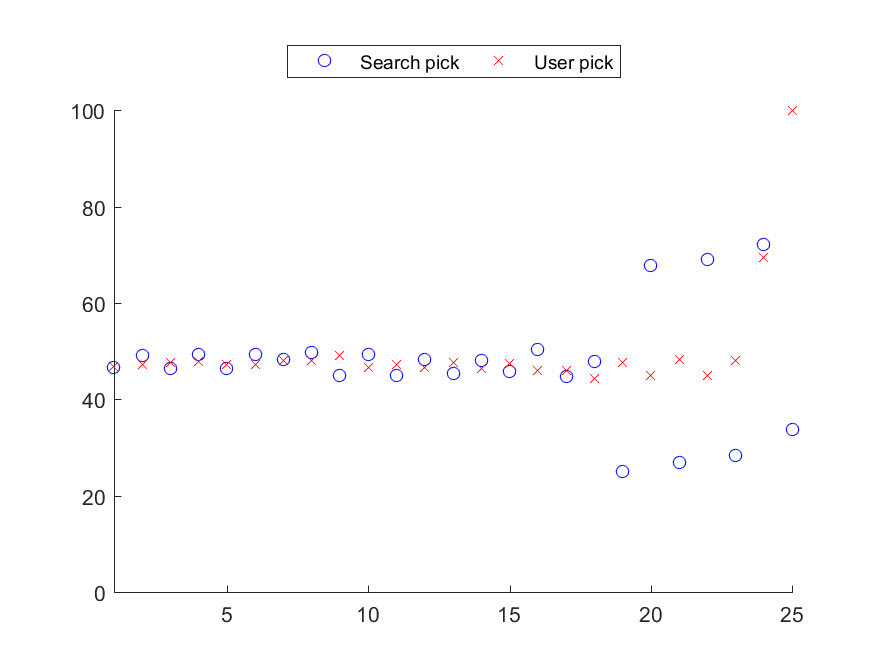
\includegraphics[scale=0.45]{figure/eval/TTTSa/evalMatchnbttt2}}
    \quad
    \subfloat[][Sanguine - NBTTT - Match 9]{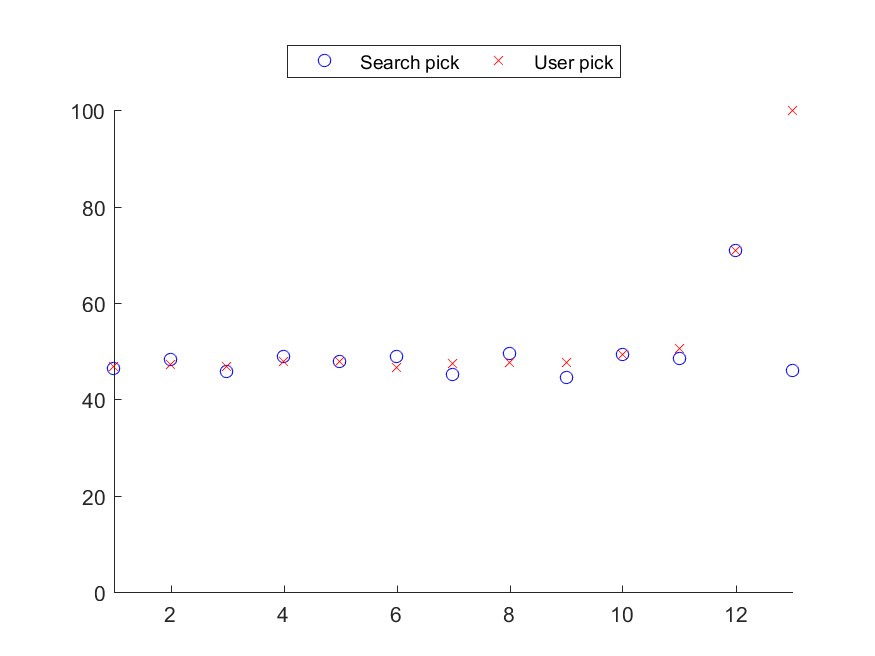
\includegraphics[scale=0.45]{figure/eval/TTTSa/evalMatchnbttt9}}
     \quad
    \subfloat[][Sanguine - NBTTT - Match 19]{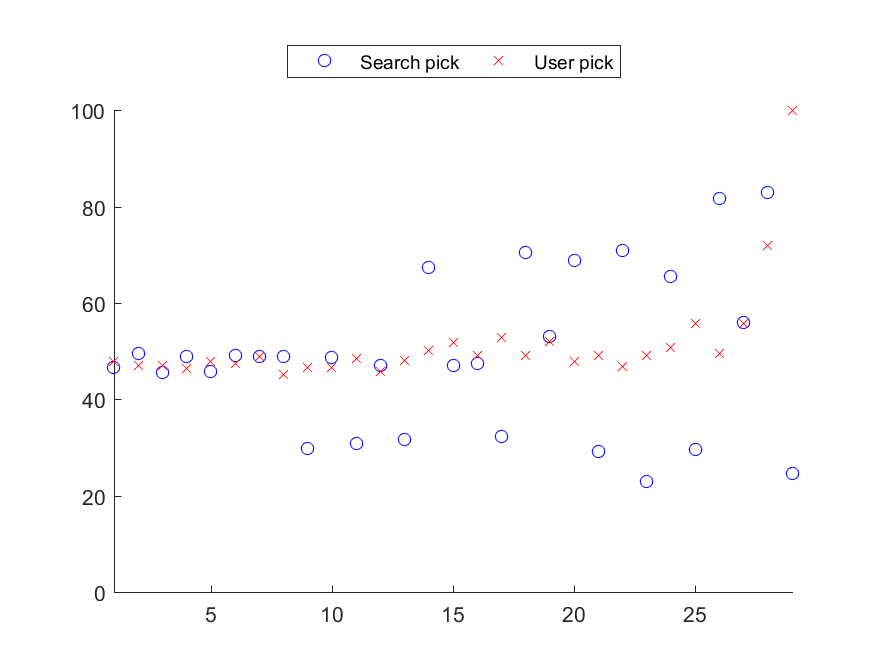
\includegraphics[scale=0.45]{figure/eval/TTTSa/evalMatchnbttt19}}
  \captionsetup{justification=centering}
    \caption{Evaluation of Nine Boards Tic-Tac-Toe for Sanguine personality.}
    \label{fig:nbtsa}
\end{figure}
In figure \ref{fig:nbtsa} can be seen three examples of tendency of game development, for the Sanguine personality, in games of Nine Boards Tic-Tac-Toe (NBTTT): figure (a) represents a mostly matching game, with divergence in the last states; figure (b) indicates more correlation between the search and the user's selection; finally, figure (c) shows a totally scattered selection. This can indeed mean that a few of those games were played by users with Sanguine personality, while others are related to other sets of parameters, therefore, another personality type.\\
Looking at the single matches, for both Nine Boards Tic-Tac-Toe and Connect Four, in figures \ref{fig:nbtttsa}, \ref{fig:nbtttph}, \ref{fig:nbtttme}, \ref{fig:nbtttch}, \ref{fig:c4sa}, \ref{fig:c4ph}, \ref{fig:c4me}, and \ref{fig:c4ch}, it can be noticed that Choleric and Sanguine tend to be a better fit. This implies that those two personalities might be easier to mimic, as well as that the personality model used in this thesis is not truly representative.\\
From figure \ref{fig:checkerseval}, presenting the results for the Checkers game, it can be seen that it has some of the Skirmish behaviour. Due to Checkers extensive state space, the difference in value between them is minimal. However, the Melancholic personality's search seems to have more difficulties matching the users', then the other personalities, confirming once more what said earlier about personalities that are easier to represent.
\begin{figure}[H]
\centering
	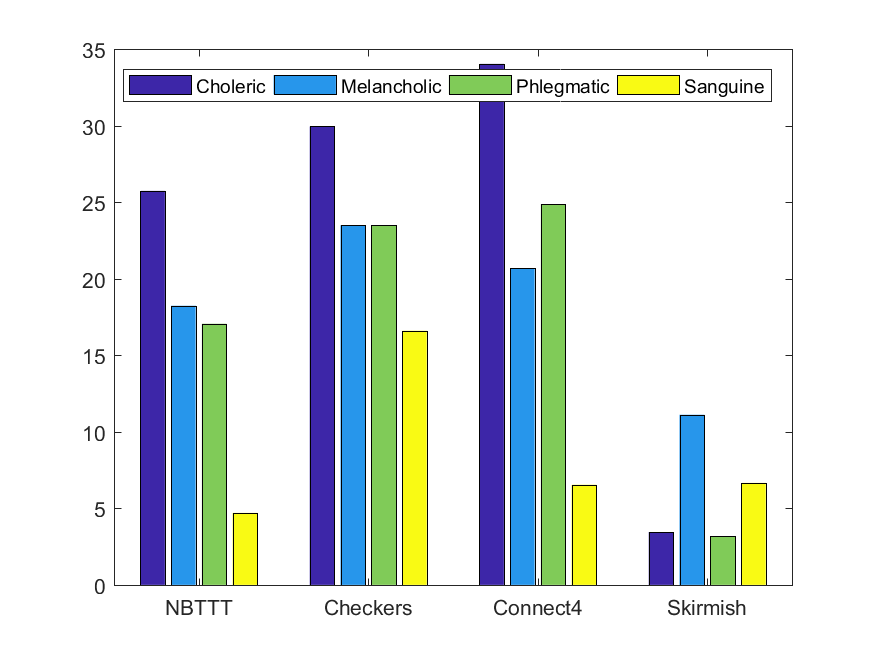
\includegraphics[scale=0.6]{figure/eval/Tot}
    \caption{Evaluation with Fittest Individuals (percent).}
    \label{fig:tot}
\end{figure}
Recapitulating, in figure \ref{fig:tot} is the summary of the Action Agreement Ratio for each game, once the search has been fed with the parameters from the genetic algorithm. It has to be pointed out that figure \ref{fig:tot} only includes the perfectly matching actions chosen by both the search and the users, while the graph in figure \ref{fig:skirmishE} only compares the moves' QValues. It is to be noticed that the Choleric parameters obtained from $25\%$ to $35\%$ matching moves, while Sanguine only $15\%$ in the best case. However, looking at figure \ref{fig:skirmishE}, it would look like more. That means that the actions chosen by the search is extremely similar in QValue to the one picked by the human player. Therefore, that might imply that the choice between the two moves is equivalent, and still achieve a human-like gaming style. 
\subsection{Skirmish Games with Random Individuals}\label{sec:skirmishrandom}
The skirmish games that had been collected, and associated to a personality, have also been tested with 3 random sets of parameters. In figure \ref{fig:randomSkirmish} is an extract of the graphs collected, showing how the behaviour of the search changes, on the same match, depending on the parameters plugged in. We found irrelevant to show the graphs relative the rest of the matches for Melancholic and Sanguine, as the behaviour is tendentiously the same as the one showed in figure \ref{fig:randomSkirmish}.
\begin{figure}[h]
\centering
    \subfloat[][Choleric Match 1 - Random Individual 1] {\includegraphics[scale=0.35]{figure/eval/rand/evalMatchskirCh1}}
    \subfloat[][Choleric Match 1 - Random Individual 2] {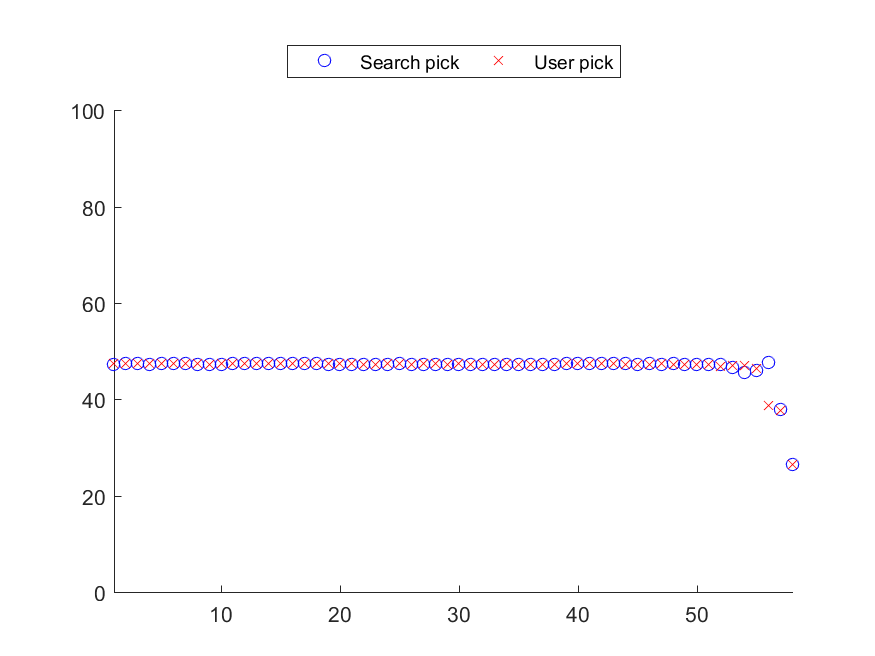
\includegraphics[scale=0.35]{figure/eval/rand/evalMatchskirCh2}}
    \subfloat[][Choleric Match 1 - Random Individual 3] {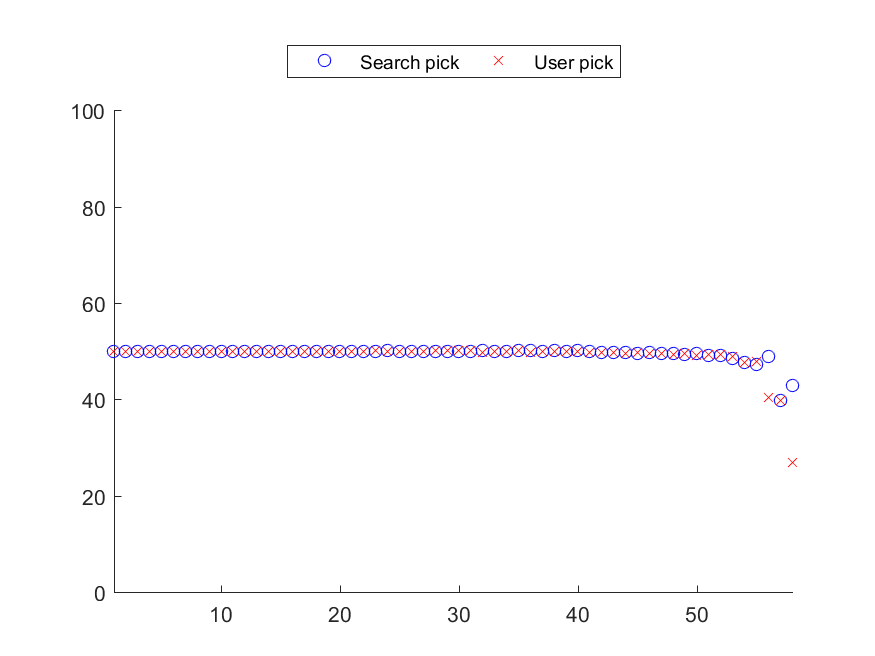
\includegraphics[scale=0.35]{figure/eval/rand/evalMatchskirCh3}}
    \qquad
    \subfloat[][Melancholic Match 1 - Random Individual 4]{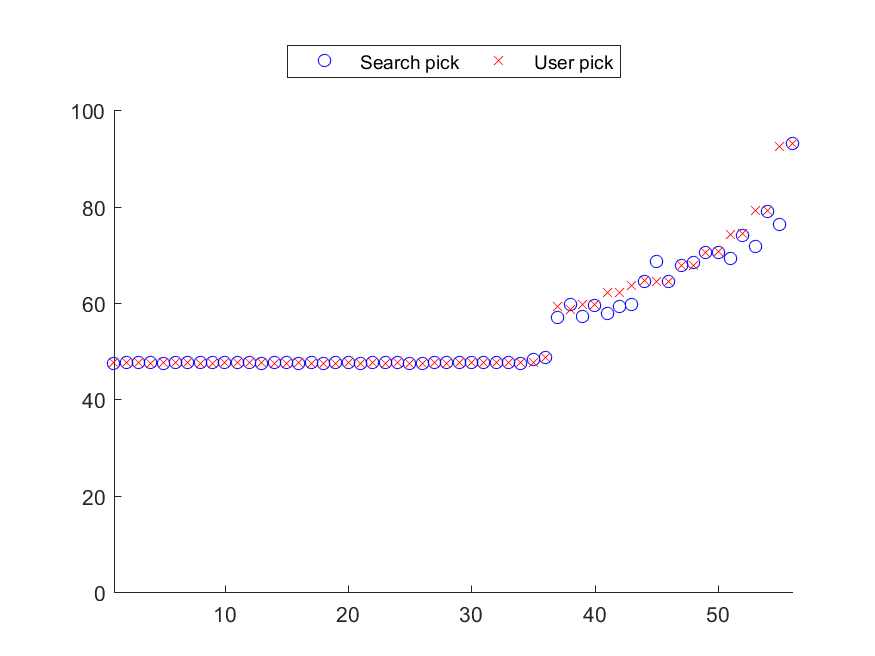
\includegraphics[scale=0.35]{figure/eval/rand/evalMatchskirMe1}}
    \subfloat[][Melancholic Match 1 - Random Individual 5]{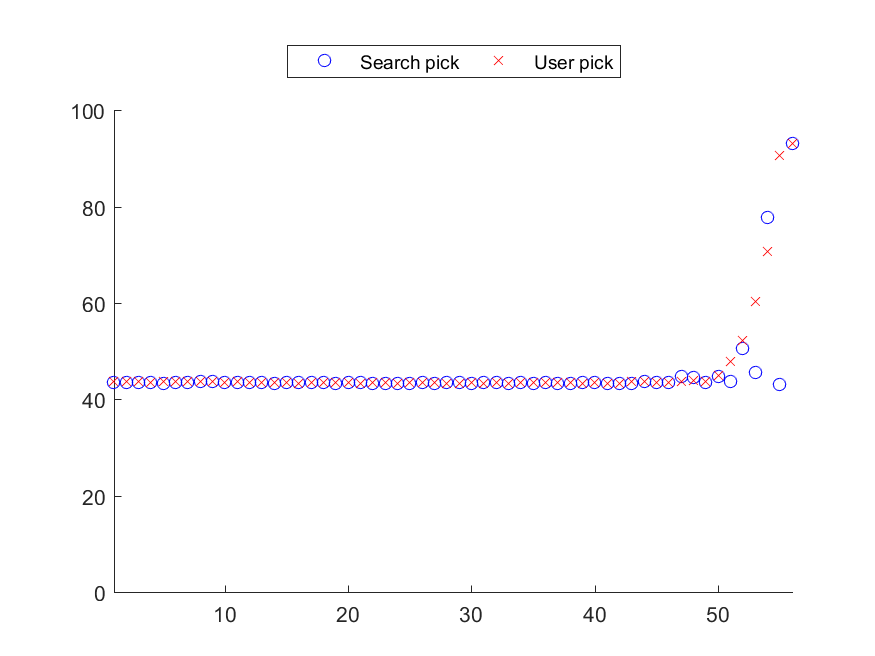
\includegraphics[scale=0.35]{figure/eval/rand/evalMatchskirMe4}}
    \subfloat[][Melancholic Match 1 - Random Individual 6]{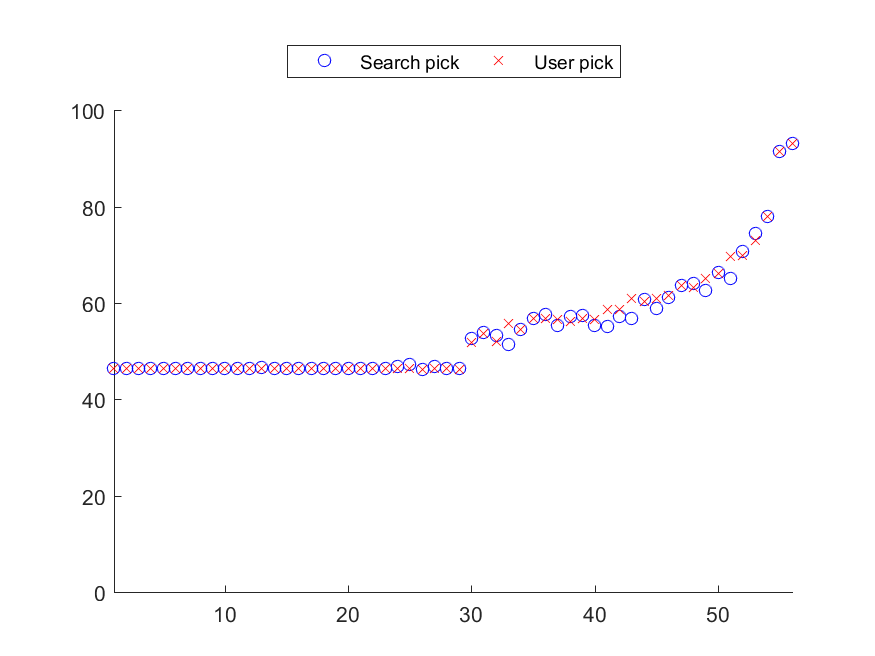
\includegraphics[scale=0.35]{figure/eval/rand/evalMatchskirMe7}}
    \qquad
    \subfloat[][Sanguine Match 1 - Random Individual 7]{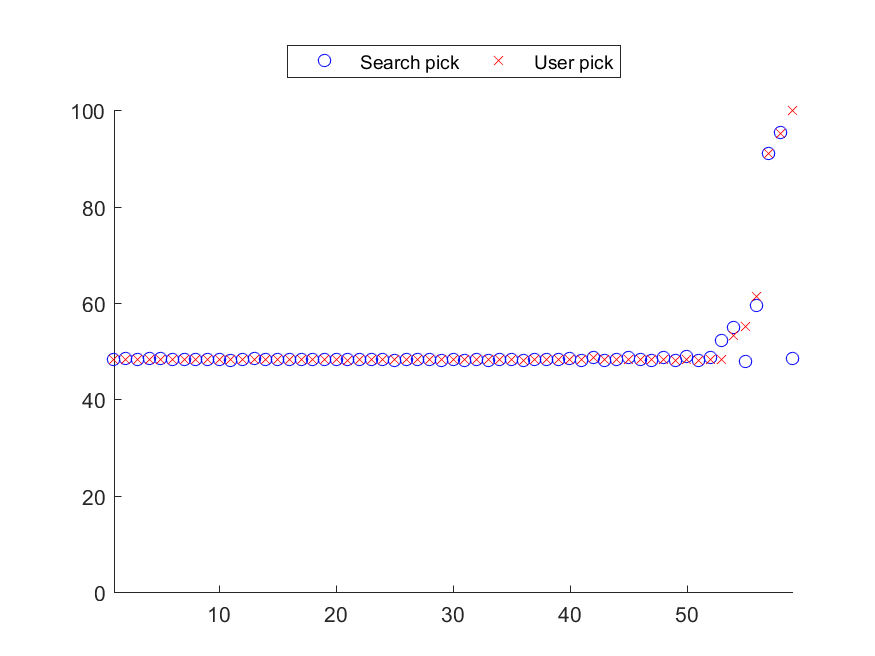
\includegraphics[scale=0.35]{figure/eval/rand/evalMatchskirSa1}}
	\subfloat[][Sanguine Match 1 - Random Individual 8]{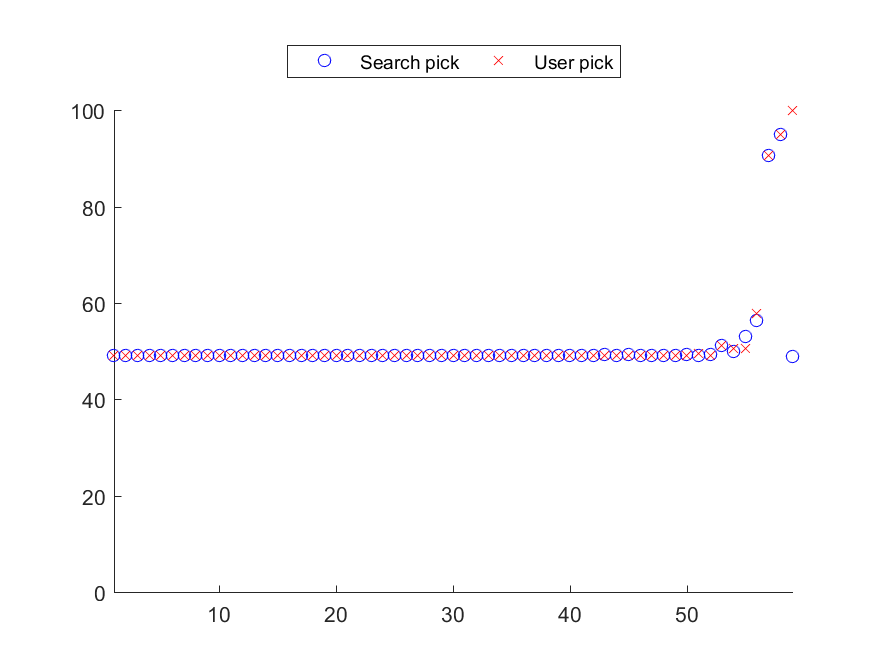
\includegraphics[scale=0.35]{figure/eval/rand/evalMatchskirSa4}}
	\subfloat[][Sanguine Match 1 - Random Individual 9]{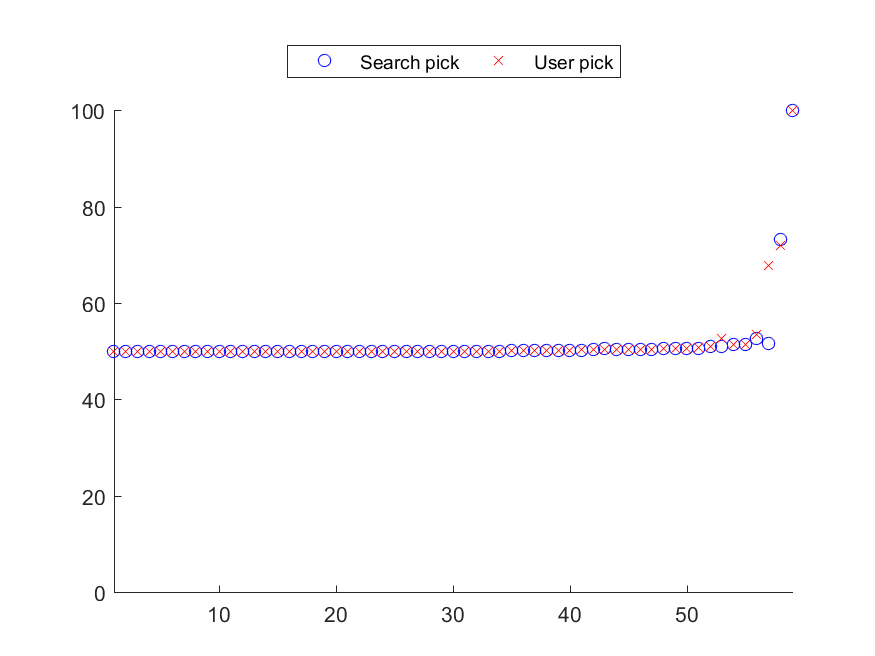
\includegraphics[scale=0.35]{figure/eval/rand/evalMatchskirSa7}}
	\qquad
    \subfloat[][Phlegmatic Match 1 - Random Individual 10]{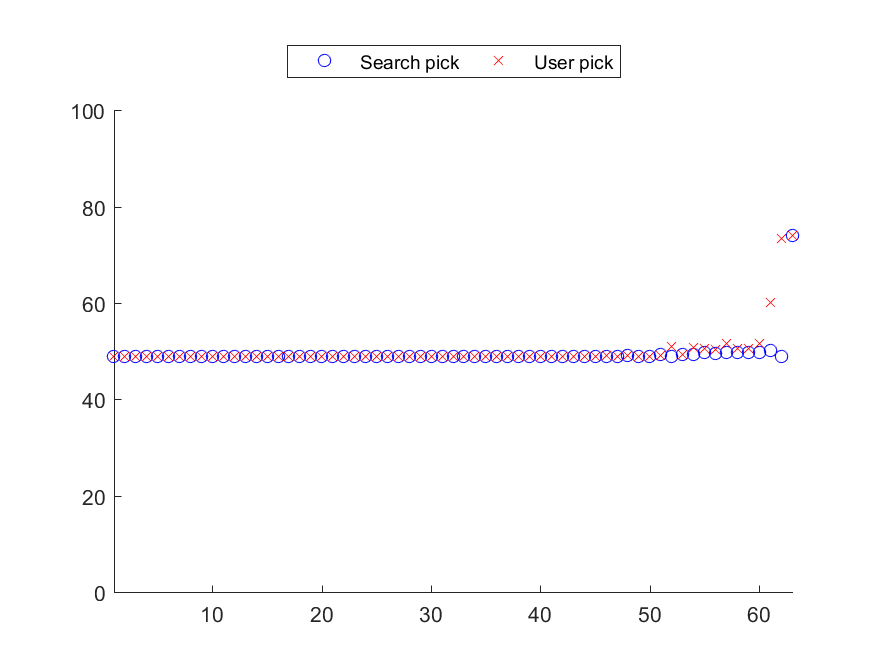
\includegraphics[scale=0.35]{figure/eval/rand/evalMatchskirPh1}}
    \subfloat[][Phlegmatic Match 1 - Random Individual 11]{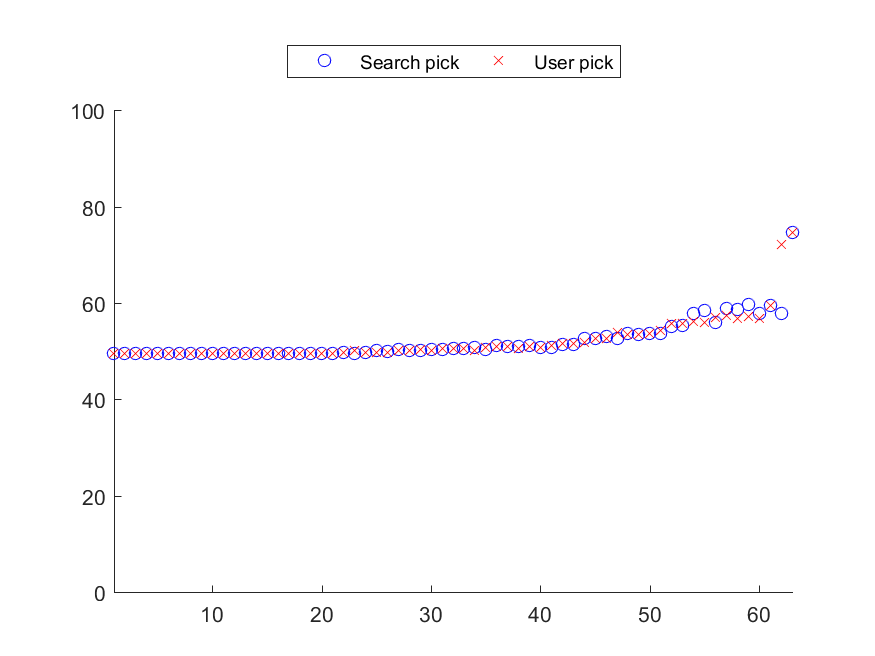
\includegraphics[scale=0.35]{figure/eval/rand/evalMatchskirPh2}}
    \subfloat[][Phlegmatic Match 1 - Random Individual 12]{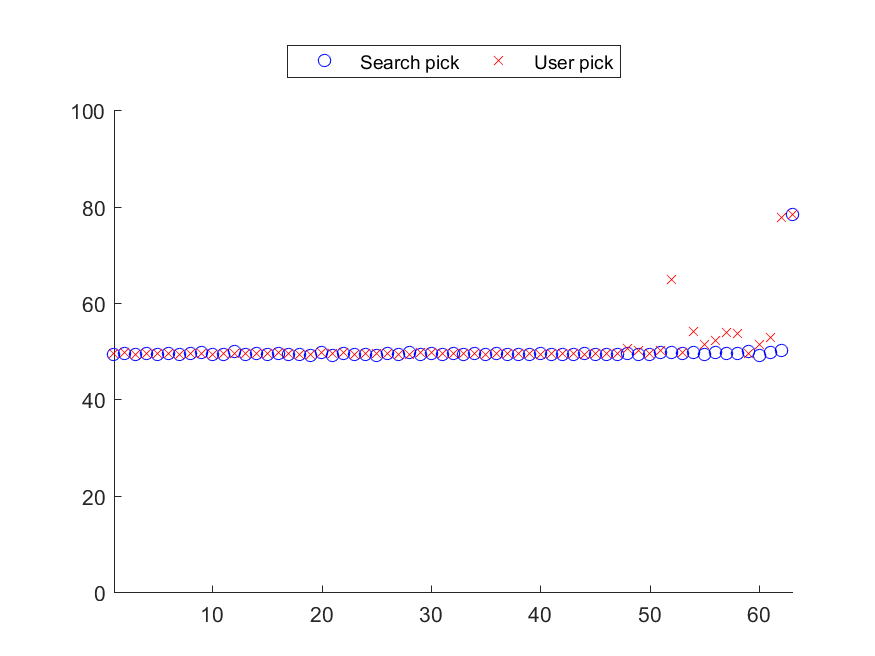
\includegraphics[scale=0.35]{figure/eval/rand/evalMatchskirPh3}}
    \caption{Evaluation of the Skirmish games with random individuals.}
    \label{fig:randomSkirmish}
\end{figure}
The individuals used have the values shown in table \ref{tab:random}.
\begin{table}[H]
	\caption{Random individuals picked for evaluation.}
    \centering
    \resizebox{\textwidth}{!}{%
    \begin{tabular}{|c|c|c|c|c|c|c|c|c|c|c|c|c|}
    \hline
Parameter & Ind. 1 & Ind. 2 & Ind. 3 & Ind. 4 & Ind. 5 & Ind. 6 & Ind. 7 & Ind. 8 & Ind. 9 & Ind. 10 & Ind. 11 & Ind. 12\\
        \hline
    eps. & 0.299 & 0.540 & 0.205 & 0.206 & 0.617 & 0.191 & 0.757 & 0.778 & 0.292 & 0.308 & 0.155 & 0.394\\
        \hline
    rave & 4508& 1464 & 4904 & 4798 & 285 & 3867 & 3223 & 3778 & 3455 &3818 & 3332 & 4852\\
        \hline
    grave & 88 & 9 & 69 & 117 & 90 & 97 & 67 & 29 & 73 & 15 & 45 & 8\\
        \hline
    chargeDis. &  0.928 & 0.945 & 0.950 & 0.989 & 0.996 & 0.984 & 0.980 & 0.901 & 0.923 & 0.931 & 0.964 & 0.995\\ 
        \hline
    treeDis. & 0.971 & 0.958 & 0.925 & 0.987 & 0.945 & 0.965 & 0.934 & 0.964 & 0.930 & 0.972 & 0.902 & 0.978\\
        \hline
    aggr. & 0.784 & 2.612 & 2.927 & 2.044 & 0.430 & 1.634 & 2.684 & 0.139 & 1.936 & 0.701 & 0.907 & 2.172\\ 
        \hline
    defen. & 1.500 & 1.866 & 1.052 & 1.316 & 0.946 & 0.645 & 1.956 & 1.503 & 0.995 & 1.075 & 0.123 & 2.998\\ 
        \hline
    ch.Depth & 65 & 20 & 94 & 60 & 19 & 67 & 34.248 & 21.756 & 62.990 & 29.706 & 75.676 & 30.799\\ 
        \hline
    horizon & 9 & 7 & 2 & 6 & 17 & 17 & 15 & 19 & 8 & 3 & 3 & 13\\
        \hline
    randErr & 0.290 & 0.485 & 0.248 & 0.754 & 0.075 & 0.392 & 0.427 & 0.624 & 0.450 & 0.095 & 0.566 & 0.024\\
        \hline
    ch.Default & 39.706 & 37.803 & 39.729 & 42.191 & 41.370 & 37.540 & 42.251 & 39.168 & 44.157 & 38.380 & 38.980 & 44.756\\
        \hline
    expl.Fac. & 125 & 81 & 120 & 49 & 36 & 35 & 5 & 13 & 121 & 47 & 137 & 12\\ 
        \hline
    niceTh. & 38.448 & 49.630 & 45.040 & 8.273 & 46.950 & 28.877 & 18.790 & 61.309 &19.282 & 45.644 & 41.199 & 35.793\\
        \hline
    \end{tabular}}
    \label{tab:random}
\end{table}
Approximately, it can be seen the same behaviour as with the "correct" parameter, excused by the magnitude of the state space of the game, as discussed earlier. However, it is possible to see some sloppiness in the search selection, compared to the user's. Figure \ref{fig:skRan} shows the percentage of matching moves having random individuals playing over the matches that were associated to personalities from the data collection. 
\begin{figure}[H]
\centering
	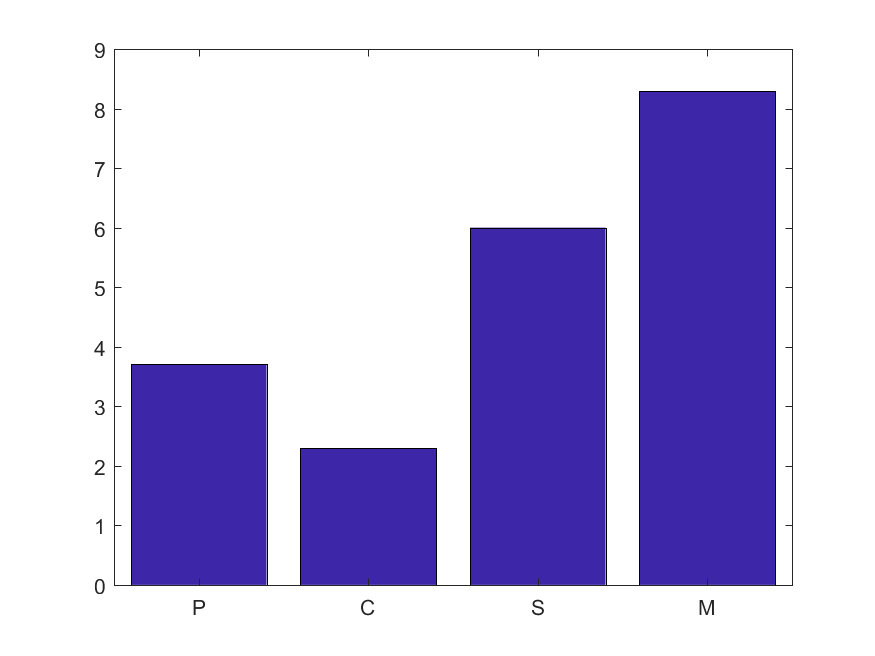
\includegraphics[scale=0.5]{figure/eval/TotRandSk}
    \caption{Actions Agreement Ratio for Skirmish games with random individuals.}
    \label{fig:skRan}
\end{figure}
This result shows an higher average of agreed moves, confirming the hypothesis of the genetic algorithm hitting a local maxima and not returning the optimal individuals, as well as that the personality model adopted might not be correctly modeled.
\subsection{Random Games with Random Individuals}\label{sec:randomrandom}
Lastly, four random individuals (A, B, C, D) have been plugged in the games we have no knowledge about, and the summary of it can be seen in figure \ref{fig:totrandom}. Comparing it with figure \ref{fig:tot}, it can be seen that individual D has more matching moves than the Choleric individual from the genetic algorithm (which was the one with the highest frequency of match, as seen in section \ref{sec:randGamesFitInd}).
\begin{figure}[H]
\centering
	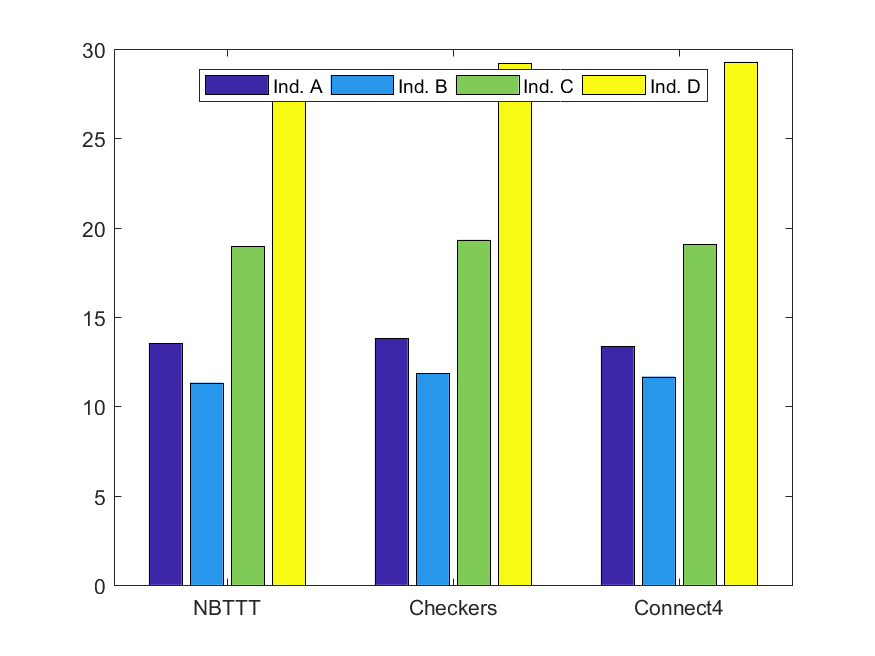
\includegraphics[scale=0.6]{figure/eval/rand/TotRand}
    \caption{Evaluation with Random Individuals (percentage).}
    \label{fig:totrandom}
\end{figure}
The meaning behind this result, in addition to what can be interpreted from the graphs in appendix \ref{sec:genegraphs}, can once more be that the personality model used for this thesis is not a true fit, as well as the genetic algorithm hit a local maxima, and would require some more tweaking to return improved results.
\section{Limitations and Improvements}
The project has been subject to limitations due to both time, and power constraints.\\
The remarkable time complexity of the Genetic Algorithm, together with time constraints, forced us to restrain the number of tests for parameters' tweaking, increasing the chances of hitting a local maxima or having premature stagnancy. More tweaking would lead to better results, overall, but we have to bound this thesis to a few choices of Genetic Algorithm parameters. It is to be recalled also that the geometric mean plotted on the graphs turned out to be slightly different than the one calculated in the genetic algorithm. Further investigations about this matter will have to be performed. In the case this would be fixed, it would be natural to suppose that the average fitness for each generation would be closer to the probability of picking one move at random, at least at initial states.\\
Mostly, however, the limitation lies on the data collection. Due to non-optimal resources, the data this thesis bases itself on, for both training and evaluation, has not been enough to infer a proper state-action distribution and get properly defined results overall. If a larger dataset would be available, it would be interesting to notice how the genetic algorithm would react to a more demanding training, and if the fittest individuals would be a better match for the personality model adopted here. In the case of more training data, it could also be possible to adopt a more detailed personality model, which could help reproducing gameplay more closely. The data to feed the genetic algorithm with will have also to be from more reliable sources, as self-assigning personality might not be accurate. Furthermore, some of our players have been acting other personalities, which could have affected the data in a negative way, considering how hard it could be to suppress emotions in some cases.
Lastly, understanding how the MCTS parameters can be changed, and how they are correlated to each other would supposedly help having more precise individuals as output from the GA.
\section{Evaluation Results}
Recapitulating the results collected during the evaluation process, it can be said that the individuals returned from the genetic algorithm do not have a relevantly better match than random parameters, over games that have been divided on the basis of our personality model. However, applied to a different set of games, random individuals seem to have a better fit (as seen in section \ref{sec:randomrandom}), leading to the idea that a different personality model might be more suitable for gaming styles representation.\\
It is then confirmed from section \ref{sec:skirmishrandom} that equation (\ref{eq:thesis}) is true, however not in a too definite way. It would be ideal if the results would be more polarised.